\documentclass[a4paper]{article}

\usepackage{graphicx}
\usepackage{float}
\usepackage{amsmath}
\usepackage[margin=3cm]{geometry}
\usepackage{titlesec}
\usepackage{hyperref}

\graphicspath{{images/}}
\newcommand{\sectionbreak}{\clearpage}

%opening
\title{koda: Deep Learning-Enhanced Pipeline for Keyword Detection in Document Images} 
\author{Matteo Pellegrino, Federico Terzi}

\begin{document}

\maketitle

\begin{abstract}
This paper proposes a pipeline, KODA, suitable for keyword highlighting in document images. At its core, KODA uses a combination of edge detection, hough transform, OCR and warping to achieve the result. The study describes the custom, deep learning-based, approach for edge detection, motivated by the problems of traditional techniques and explaining the model training process, along with examples. Moreover, document detection and warping algorithms are detailed, as well as the keyword highlighting process.

\vspace{1cm}
All the code can be found in the repository: \url{https://github.com/federico-terzi/koda}
\end{abstract}

\begingroup\let\clearpage\relax
\vspace{1cm}
\tableofcontents \endgroup

\section{Introduction}
Document detection in images is a well-known problem, whose most common use-case is document scanning using mobile devices, achieving results comparable with commercial scanners. Although many apps already solve this problem, only a few offer the possibility to interactively search the document for specific keywords, a feature which could be beneficial to many people. For example, those with alimentary disorders could greatly benefit from an application which, from a simple restaurant menu or a product label picture, could show all the contained allergens conveniently.

Our proposed pipeline, KODA, is specifically designed to detect documents from images, extract all the interesting keywords and, eventually, highlight them in the original image, so that the user can conveniently see them.

The paper is organized as follows: the first section, Architecture, describes the general structure and components of KODA. In the Edge Detection section, starting from the limitations of traditional techniques, a deep learning-based approach is proposed, along with a thorough comparison. Thereafter, the Corners Detection section describes the document detection algorithm itself, exploiting Hough transformations. Then, in the Document analysis section, warping, OCR and highlighting techniques are described. Finally, the concluding remarks are drawn in the last section.

\section{Architecture}

KODA architecture was inspired by a Dropbox article \footnote{https://blogs.dropbox.com/tech/2016/08/fast-and-accurate-document-detection-for-scanning/} which defines the steps to solve a problem similar to the one this project is based on.

The process is divided into two macro tasks (Fig. \ref{fig:pipeline}): image processing and keywords detection: The former detects a document from an image and retrieve all the contained words. The latter find user specified keywords, highlighting them in the document image.

\begin{figure}[!htbp]
	\centering
	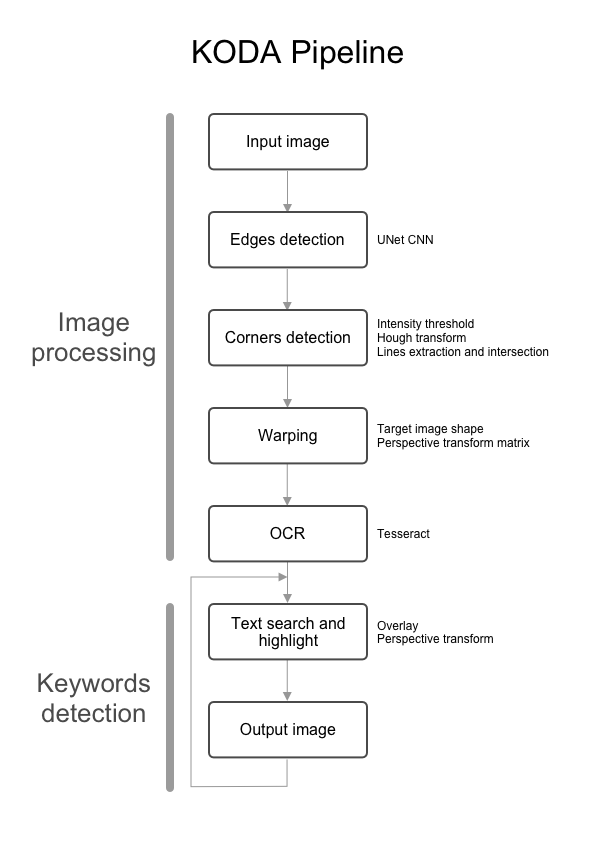
\includegraphics[width=0.8\linewidth]{Pipeline.png}
	\caption{KODA Pipeline scheme with sub-tasks. The computationally expensive processing is done once per input image, then the user can search for keywords and retrieves the output image multiple times repeatedly.}
	\label{fig:pipeline}
\end{figure}

\begin{figure}[!htbp]
	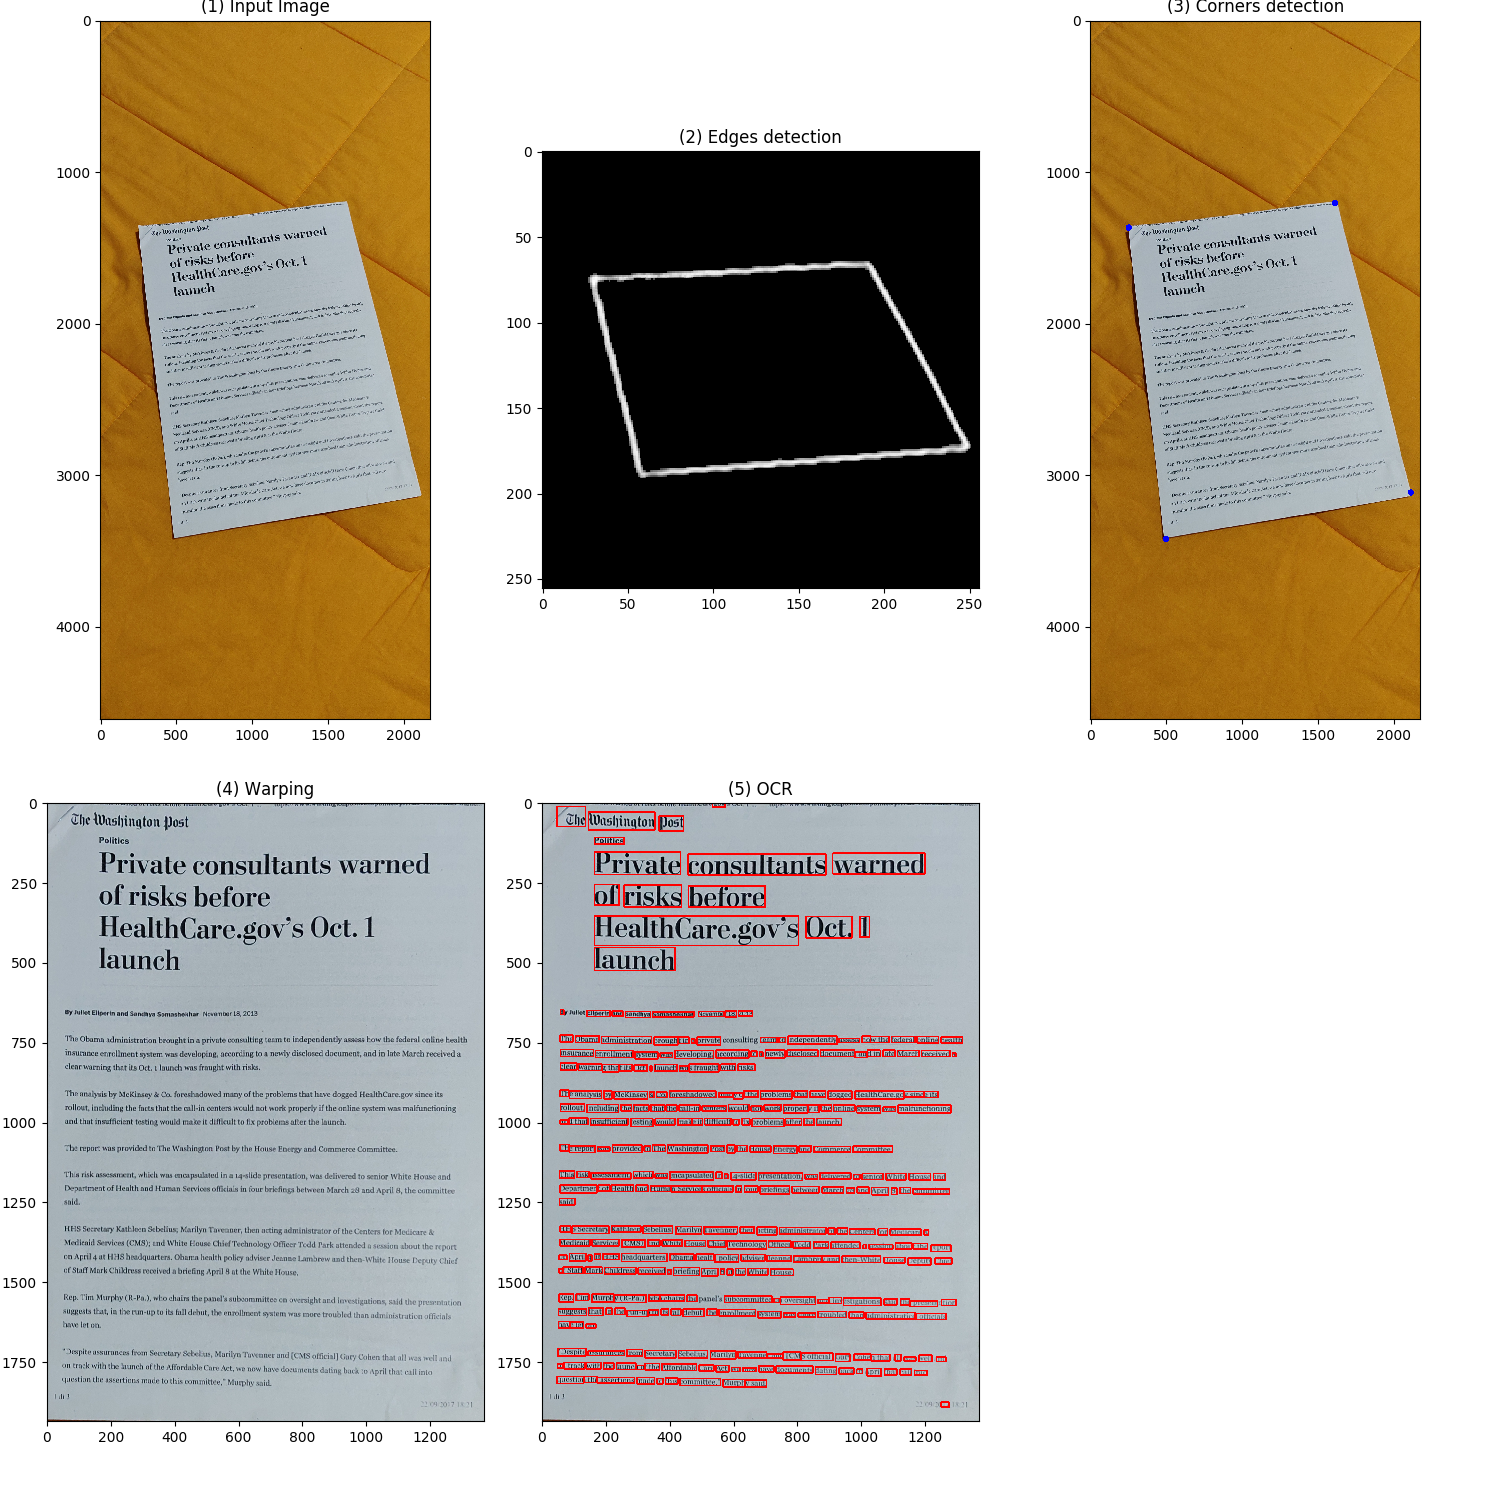
\includegraphics[width=\linewidth]{ipt.png}
	\caption{Image processing tasks example. Note: edges detection returns a resized image (256x256)}
	\label{fig:imageprocessing}
\end{figure}





\section{Edge Detection}

Above all the possible approaches, the pipeline proposed in this paper heavily
relies on edges to detect documents inside images. Therefore, in order to obtain
good results, it is crucial to employ a solid \textit{edge detection} algorithm.


\subsection{First attempts with Canny}

Our initial attempts to detect document edges involved the well known \textit{Canny edge detector} \footnote{J. Canny, "A Computational Approach to Edge Detection," in IEEE Transactions on Pattern Analysis and Machine Intelligence, vol. PAMI-8, no. 6, pp. 679-698, Nov. 1986.
	doi: 10.1109/TPAMI.1986.4767851}. 
Although applying the filter directly does detect the sheet edges, it presents many artifacts
due to the text printed on the document itself (as seen in Fig. \ref{fig:canny_gaussian} (B)).

In order to mitigate the problem, a \textit{Gaussian filter} is applied before the edge detection, obtaining a clear highlighting of the interesting edges (as seen in Fig.  \ref{fig:canny_gaussian} (C)).

\begin{figure}[!htb]
	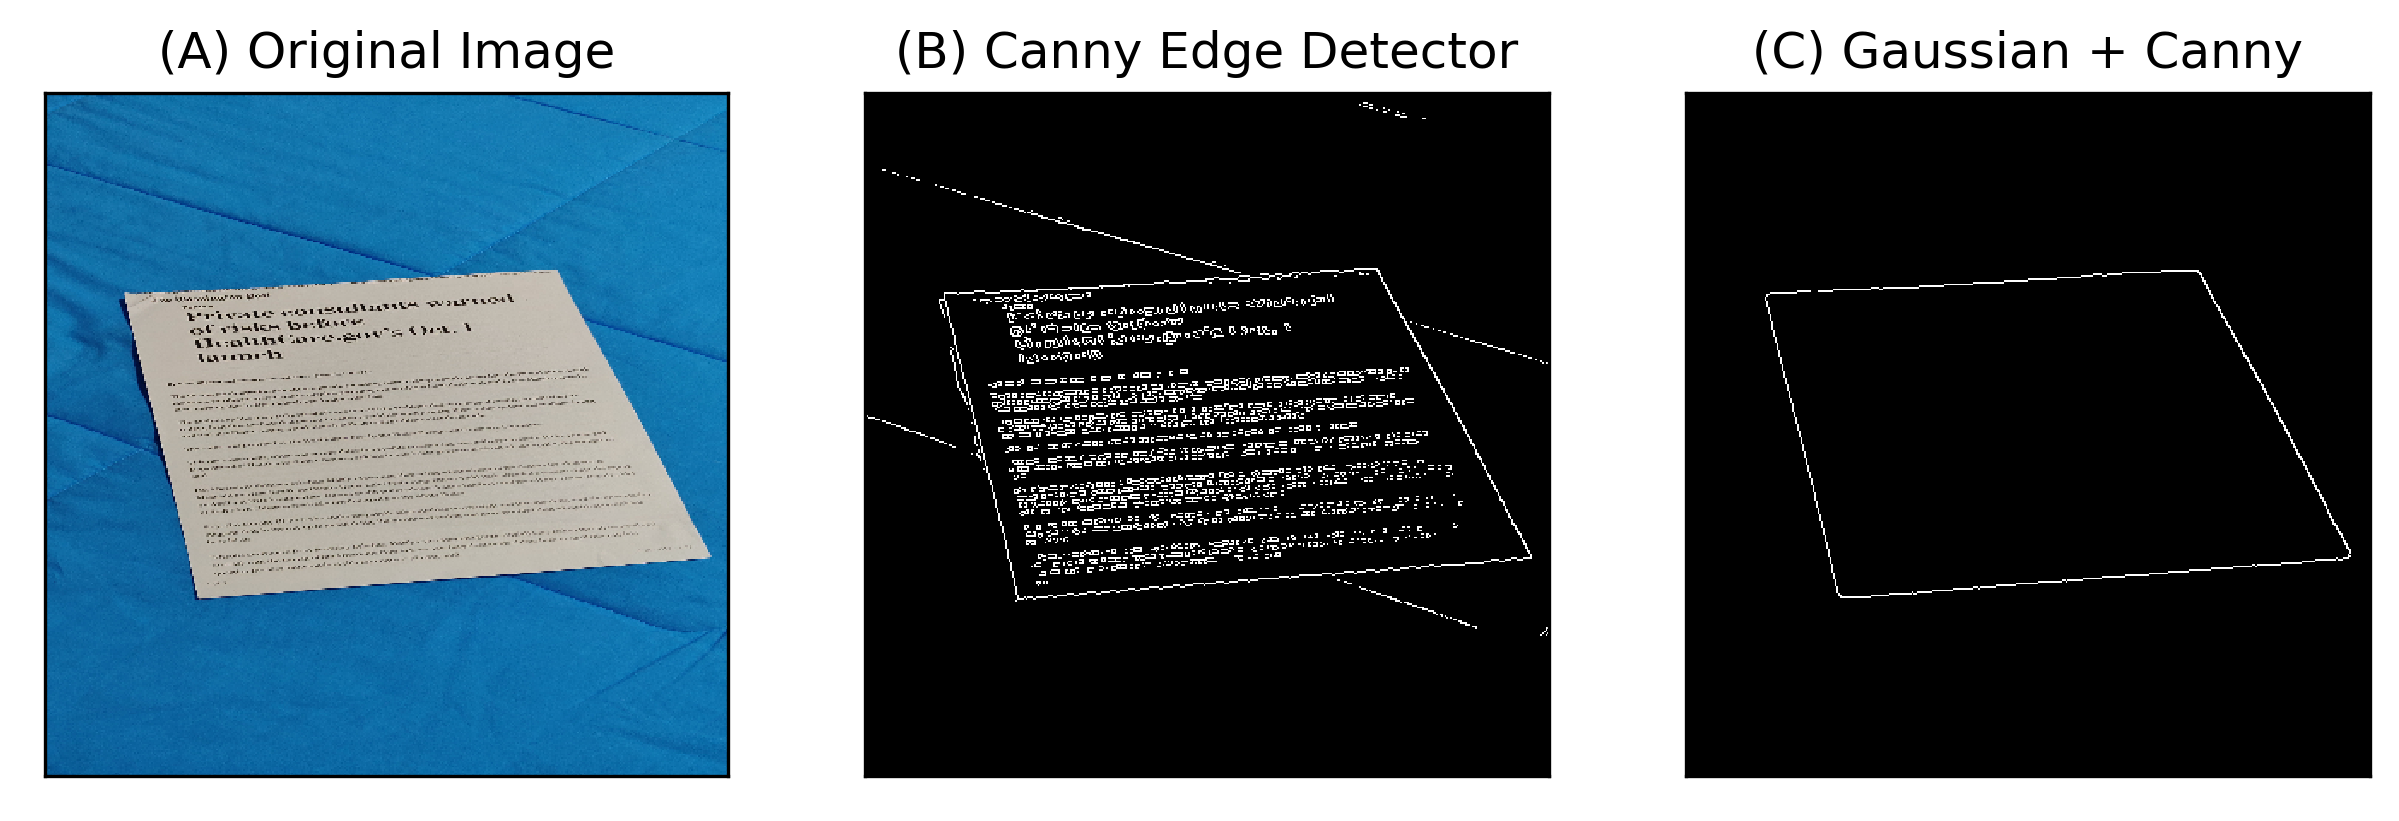
\includegraphics[width=\linewidth]{canny_gaussian.png}
	\caption{Application of Canny edge detector to the original image without/with a Gaussian Filter}
	\label{fig:canny_gaussian}
\end{figure}

Despite the result, after many observations it became clear that this approach was not robust enough to
work in all real-world scenarios. In particular, Canny's parameter tuning turned out to be a major
problem, as it can be seen in Fig \ref{fig:canny_comparison}, where a combination of parameters,
despite producing good results in some scenarios, proved itself incapable of generalizing well in others.

\begin{figure}[htb!]
	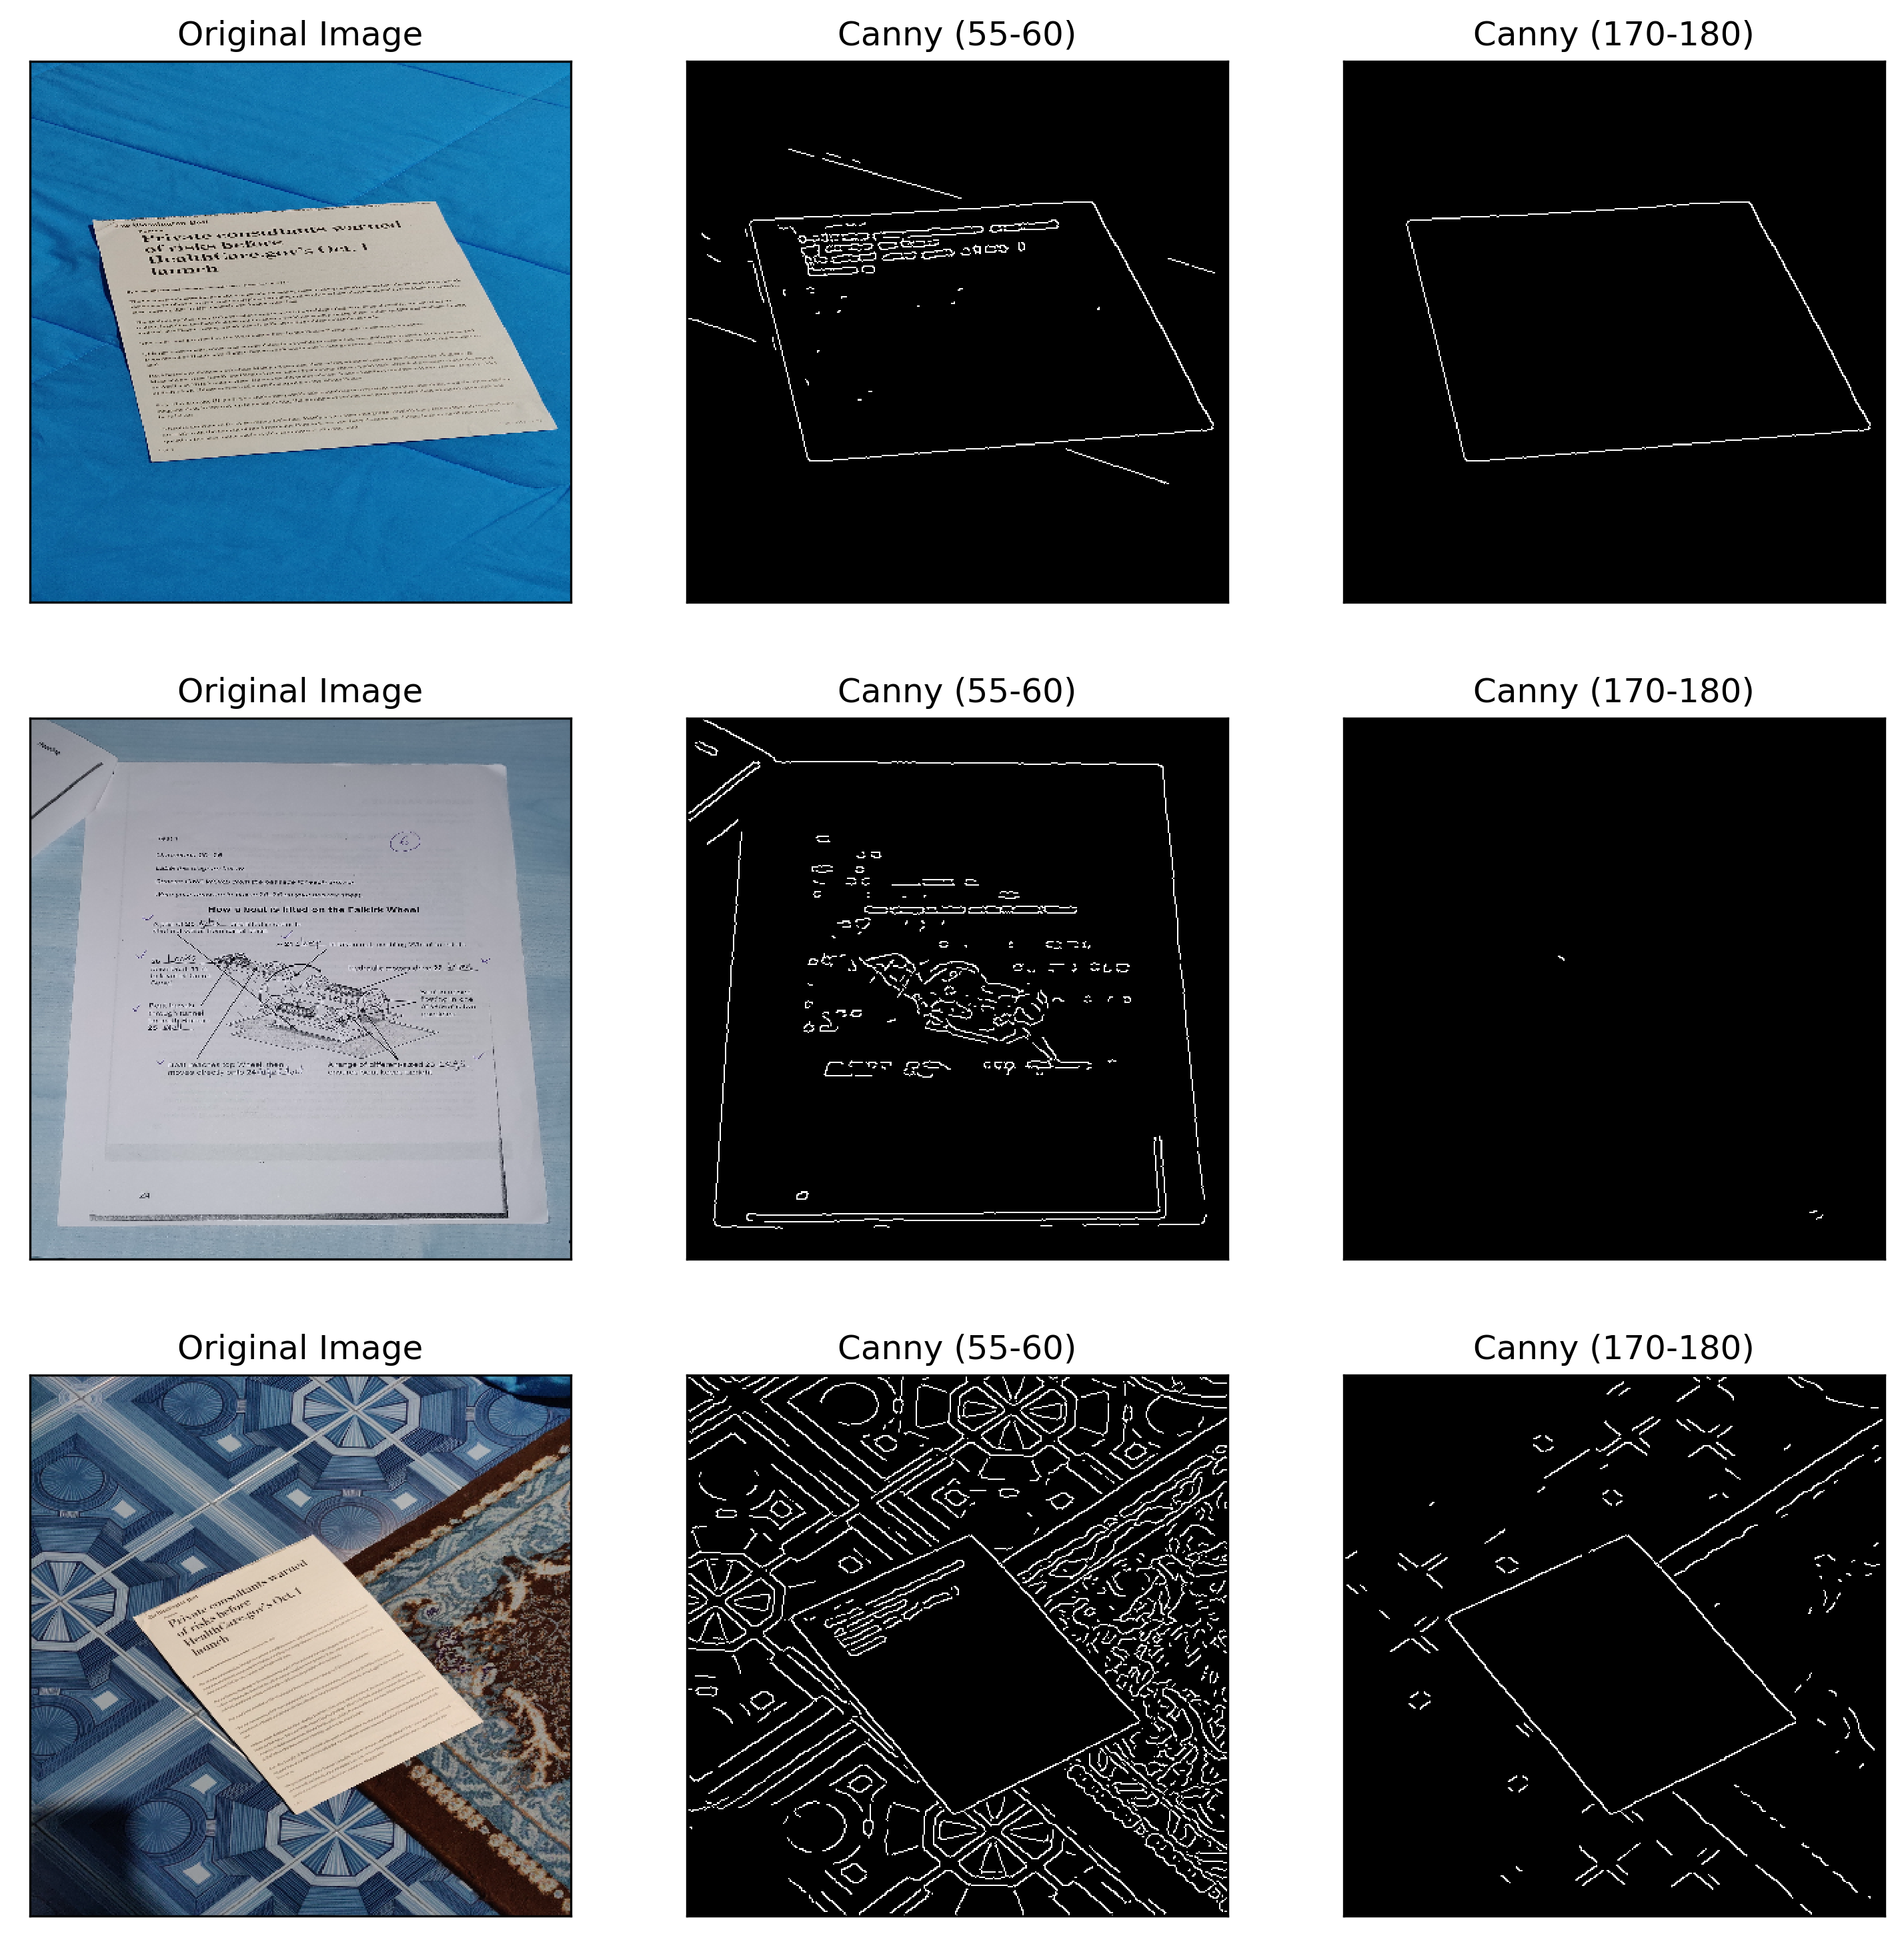
\includegraphics[width=\linewidth]{canny_comparison.png}
	\caption{Comparison of different thresholds for Canny edge detector}
	\label{fig:canny_comparison}
\end{figure}

\subsection{Deep Learning approach}

In order to make the pipeline able to deal with real-world images, it is crucial to develop an
edge detection mechanism capable of generalizing better in heterogeneous situations. 
For this reason, a \textit{Deep Learning}-based approach was explored with the aim of creating a model
capable of distinguishing document sheet edges from the rest of the image.

Due to the lack of a suitable dataset with labelled document edges, a custom one was created.
In particular, 250 images containing document sheets were taken under different lighting conditions, 
backgrounds and positions. Thereafter, every image was labelled with the 4 corner coordinates of the document.

For this particular task, \textit{Keras}, an open-source Python library for Deep Learning \footnote{https://keras.io/}, was chosen to build the model. Many experiments were made to find the right architecture, most of them 
exploiting \textit{convolutional neural networks}. Above all of them, KODA uses \textit{U-Net}
\footnote{O. Ronneberger, P. Fischer, T. Brox, "U-Net: Convolutional Networks for Biomedical Image Segmentation", CoRR, abs/1505.04597, 2015}, a popular architecture for \textit{object segmentation}, and in particular an open-source implementation for Keras \footnote{https://github.com/zhixuhao/unet}.

The model takes a 3-dimensional input image (RGB) and outputs a 2-d map of the edges. Although the shape
of those matrices can vary, KODA uses a 256 pixels side for both input and output, as it provides a reasonable compromise between size and resolution. Fig. \ref{fig:label_edge} illustrates the way a
sample is fed to the network. In particular, the input image is resized to a 256x256 RGB image and the
output label is a gray scale map of the expected document edges.

\begin{figure}[htb!]
	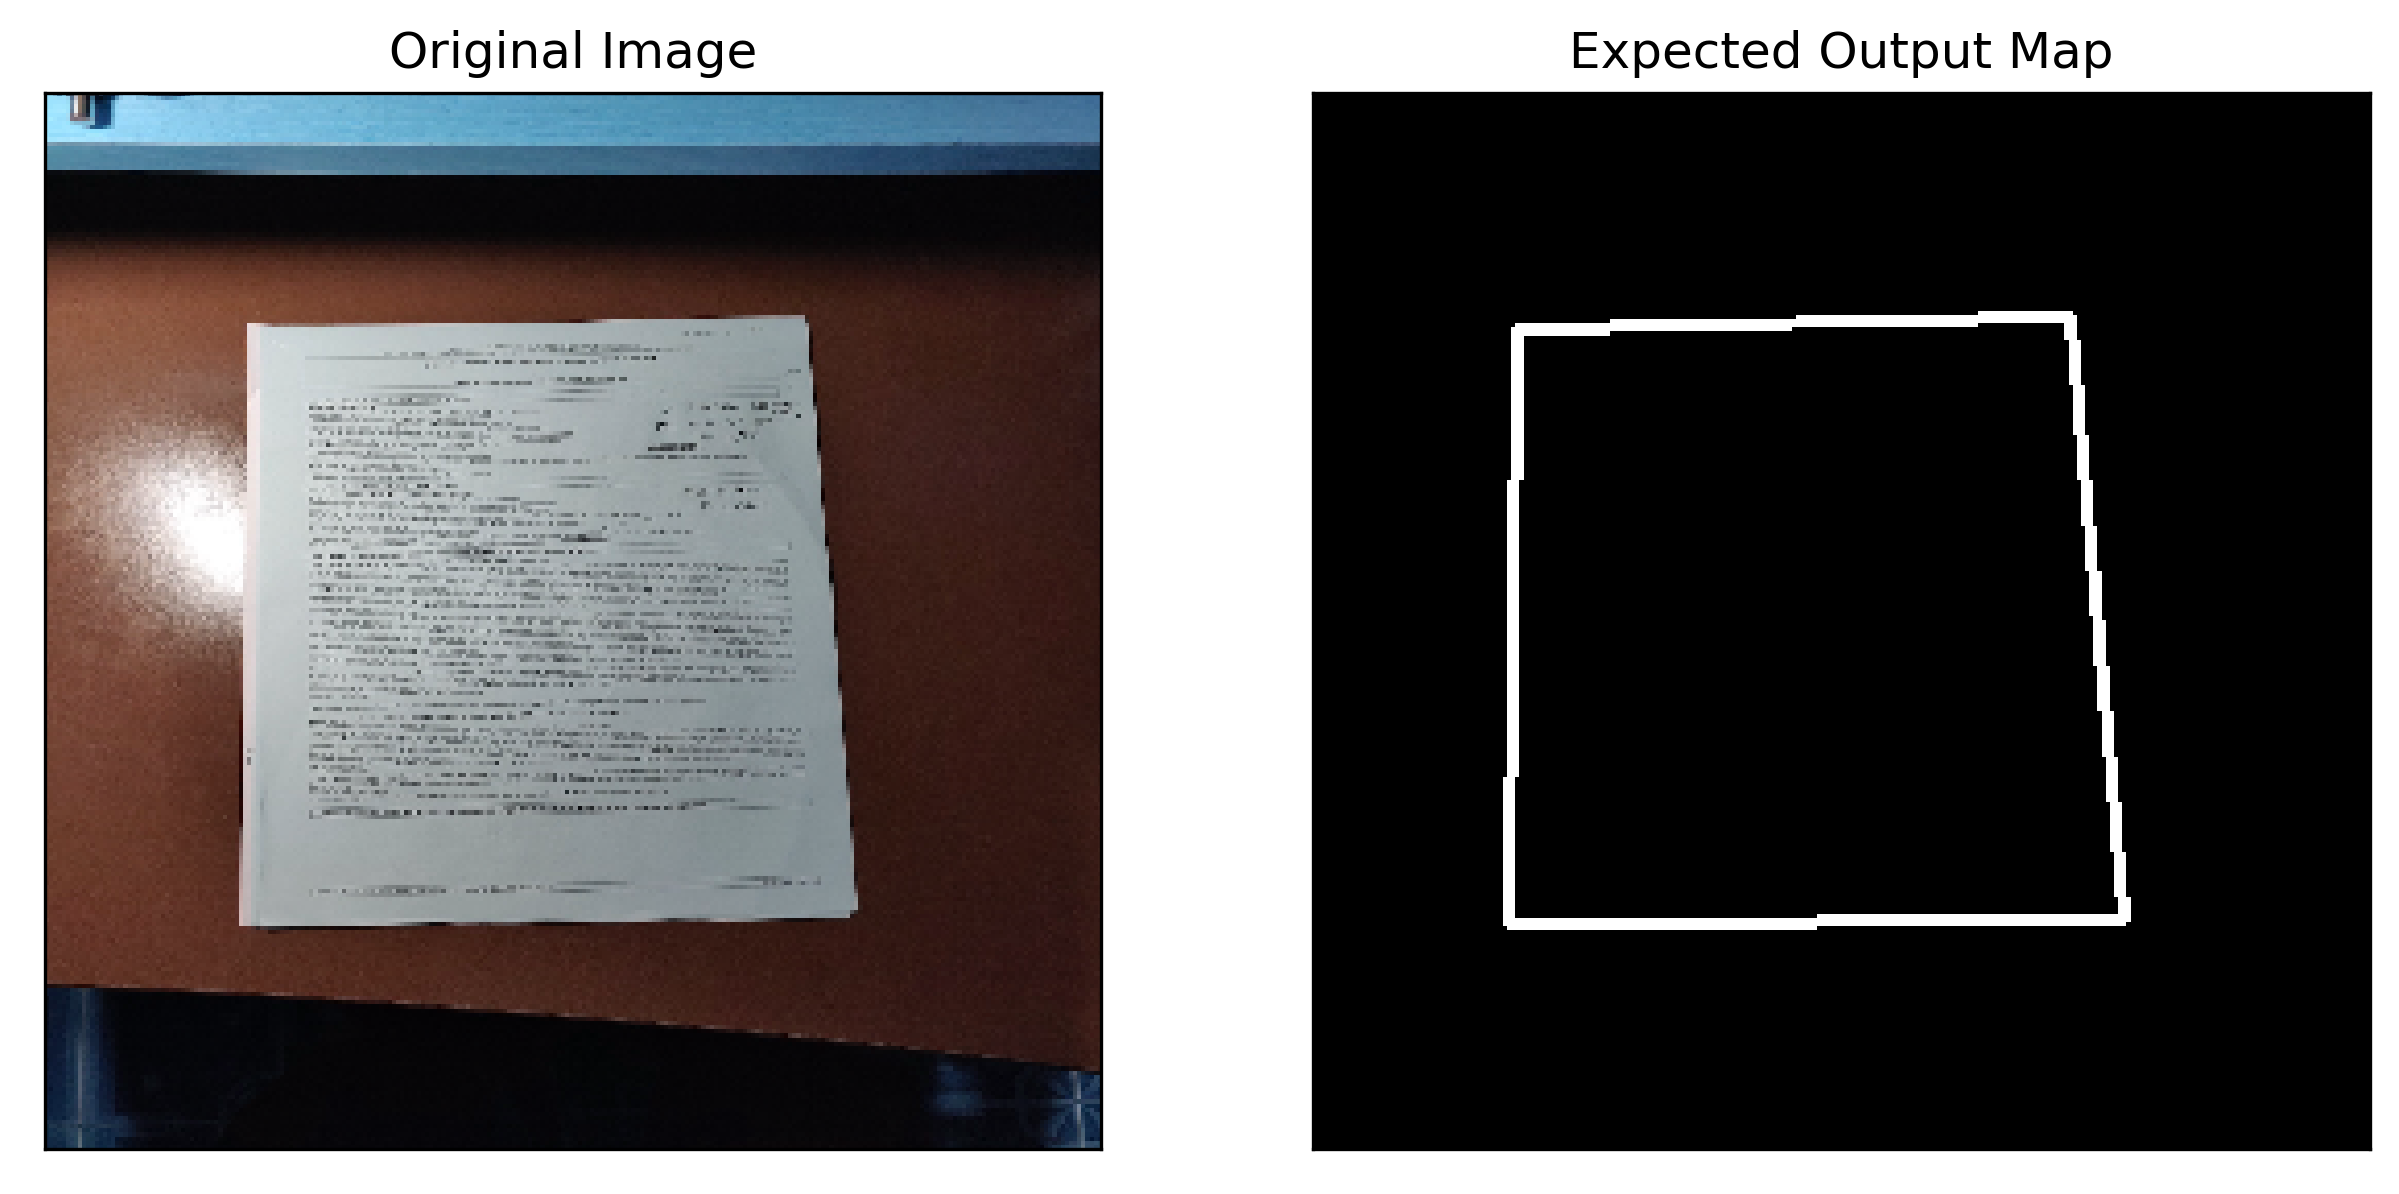
\includegraphics[width=\linewidth]{label_edge.png}
	\caption{Example of the way a sample is fed to the network.}
	\label{fig:label_edge}
\end{figure}

Due to the high number of required samples, the dataset itself is insufficient to fully train the network.
For this reason, a technique called \textit{data augmentation} is applied to provide the model
with enough variation. In particular, before being fed to the network, a random combination of transformations, such as scale, translation, rotation and brightness changes, is applied to the image and to the resulting edge feature map, as shown in Fig. \ref{fig:augmented_image}.

\begin{figure}[H]
	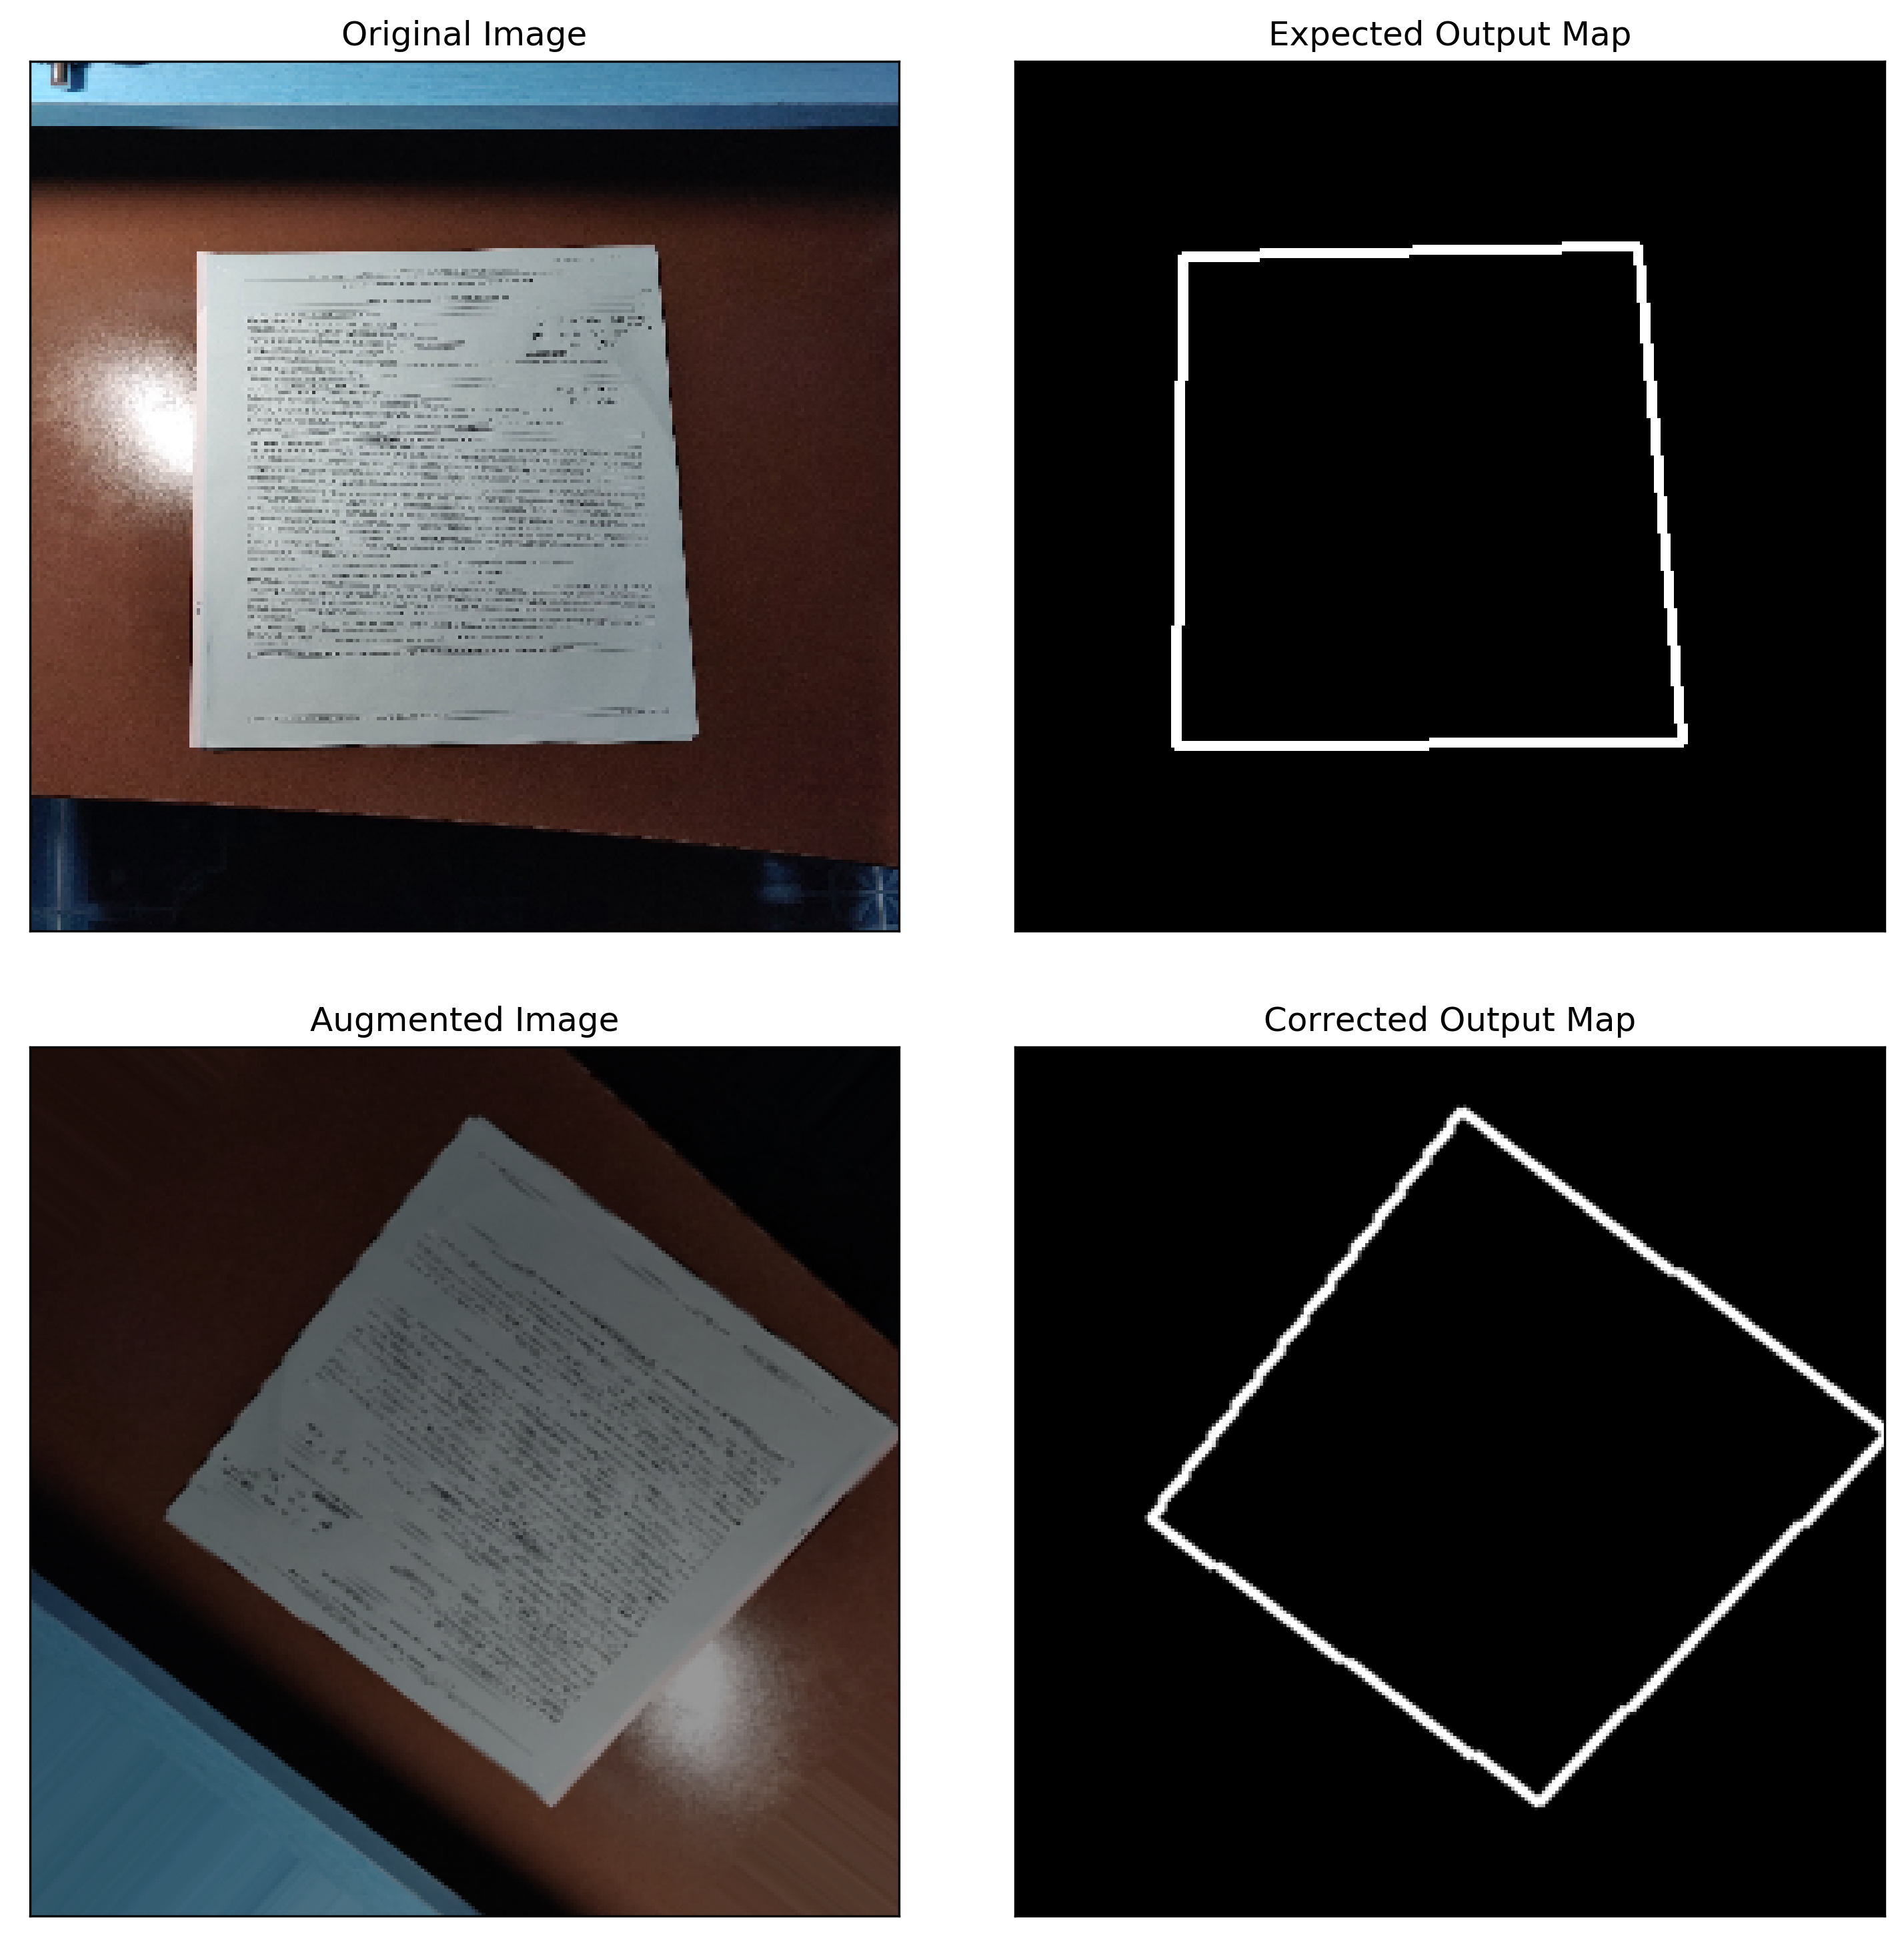
\includegraphics[width=\linewidth]{augmented_image.png}
	\caption{Example of Data Augmentation}
	\label{fig:augmented_image}
\end{figure}

During the training, finding the best compromise between good results and overfitting proved to be a challenging problem. In particular, the \textit{loss function}, in this case \textit{binary crossentropy}, 
was not representative of the model's quality. As it can be seen in Fig. \ref{fig:model_loss}, the loss value of the validation set settles around epoch 40. Despite this, further experimentation shows that the model still improves well beyond that epoch. For this reason, a new approach was needed to evaluate the performances of the model.

\begin{figure}[htb!]
	\centering
	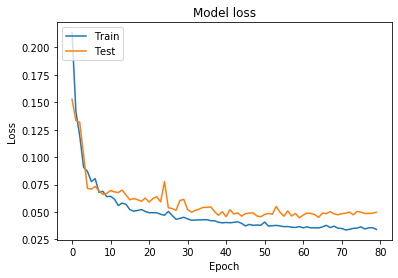
\includegraphics[width=0.7\linewidth]{model_loss.png}
	\caption{Model loss over the first 80 epochs.}
	\label{fig:model_loss}
\end{figure}

Despite being simple, the proposed solution is to save the current model's results over a set of test images after each epoch, as well as saving the model itself. This approach allows a simple comparative analysis, and allowed us to select the best model according to its actual results. Epoch 70 produced the best performing model from a generalization standpoint, while further epochs shown interesting but less effective trends. In particular, as you can see from Fig. \ref{fig:edge_comparison_epoch}, the model at epoch 70 is capable of detecting both (A) and (B) edges fairly well, whereas the one at epoch 140 presented an improved result in (A), removing uninteresting objects from the top portion of the image, but was almost incapable of recognizing edges in (B). This phenomenon could be explained as the model starting to empathize straight lines and discarding curved ones. Unfortunately, the latter are a common case and should be considered, therefore the first model was chosen.

\begin{figure}[!htbp]
	\centering
	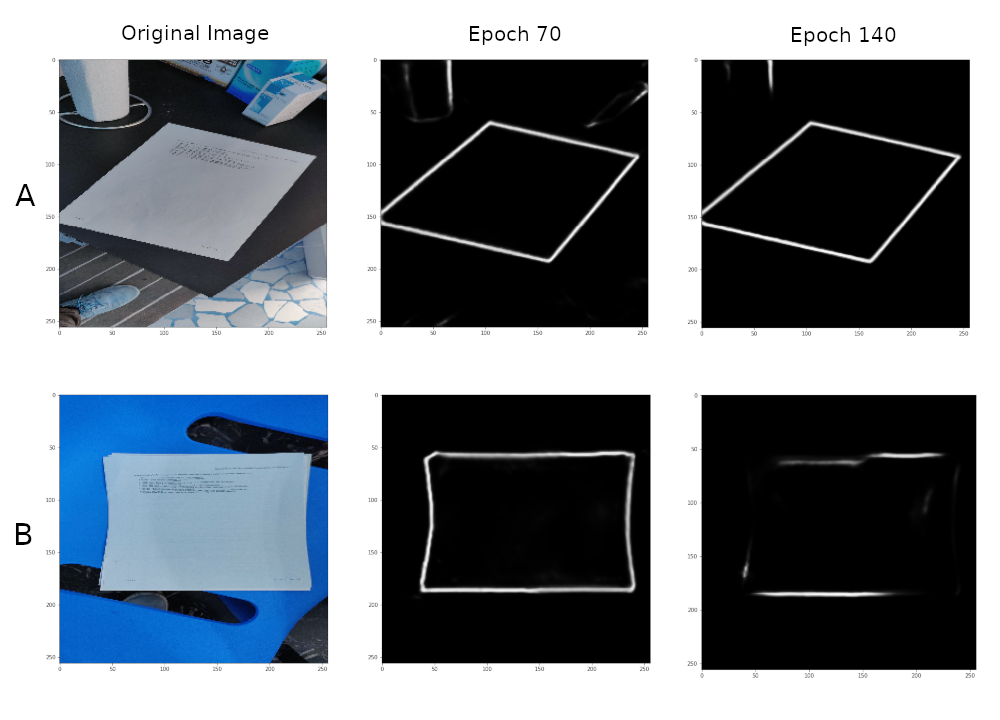
\includegraphics[width=\linewidth]{edge_comparison_epoch.png}
	\caption{Comparison of the edge detector over different epochs.}
	\label{fig:edge_comparison_epoch}
\end{figure}

\subsection{Comparison between the two approaches}

An overview of the end result can be seen in Fig. \ref{fig:deep_comparison}, which also shows a comparison with the previous Canny-based approach.

\begin{figure}[!htbp]
	\centering
	\makebox[\textwidth][c]{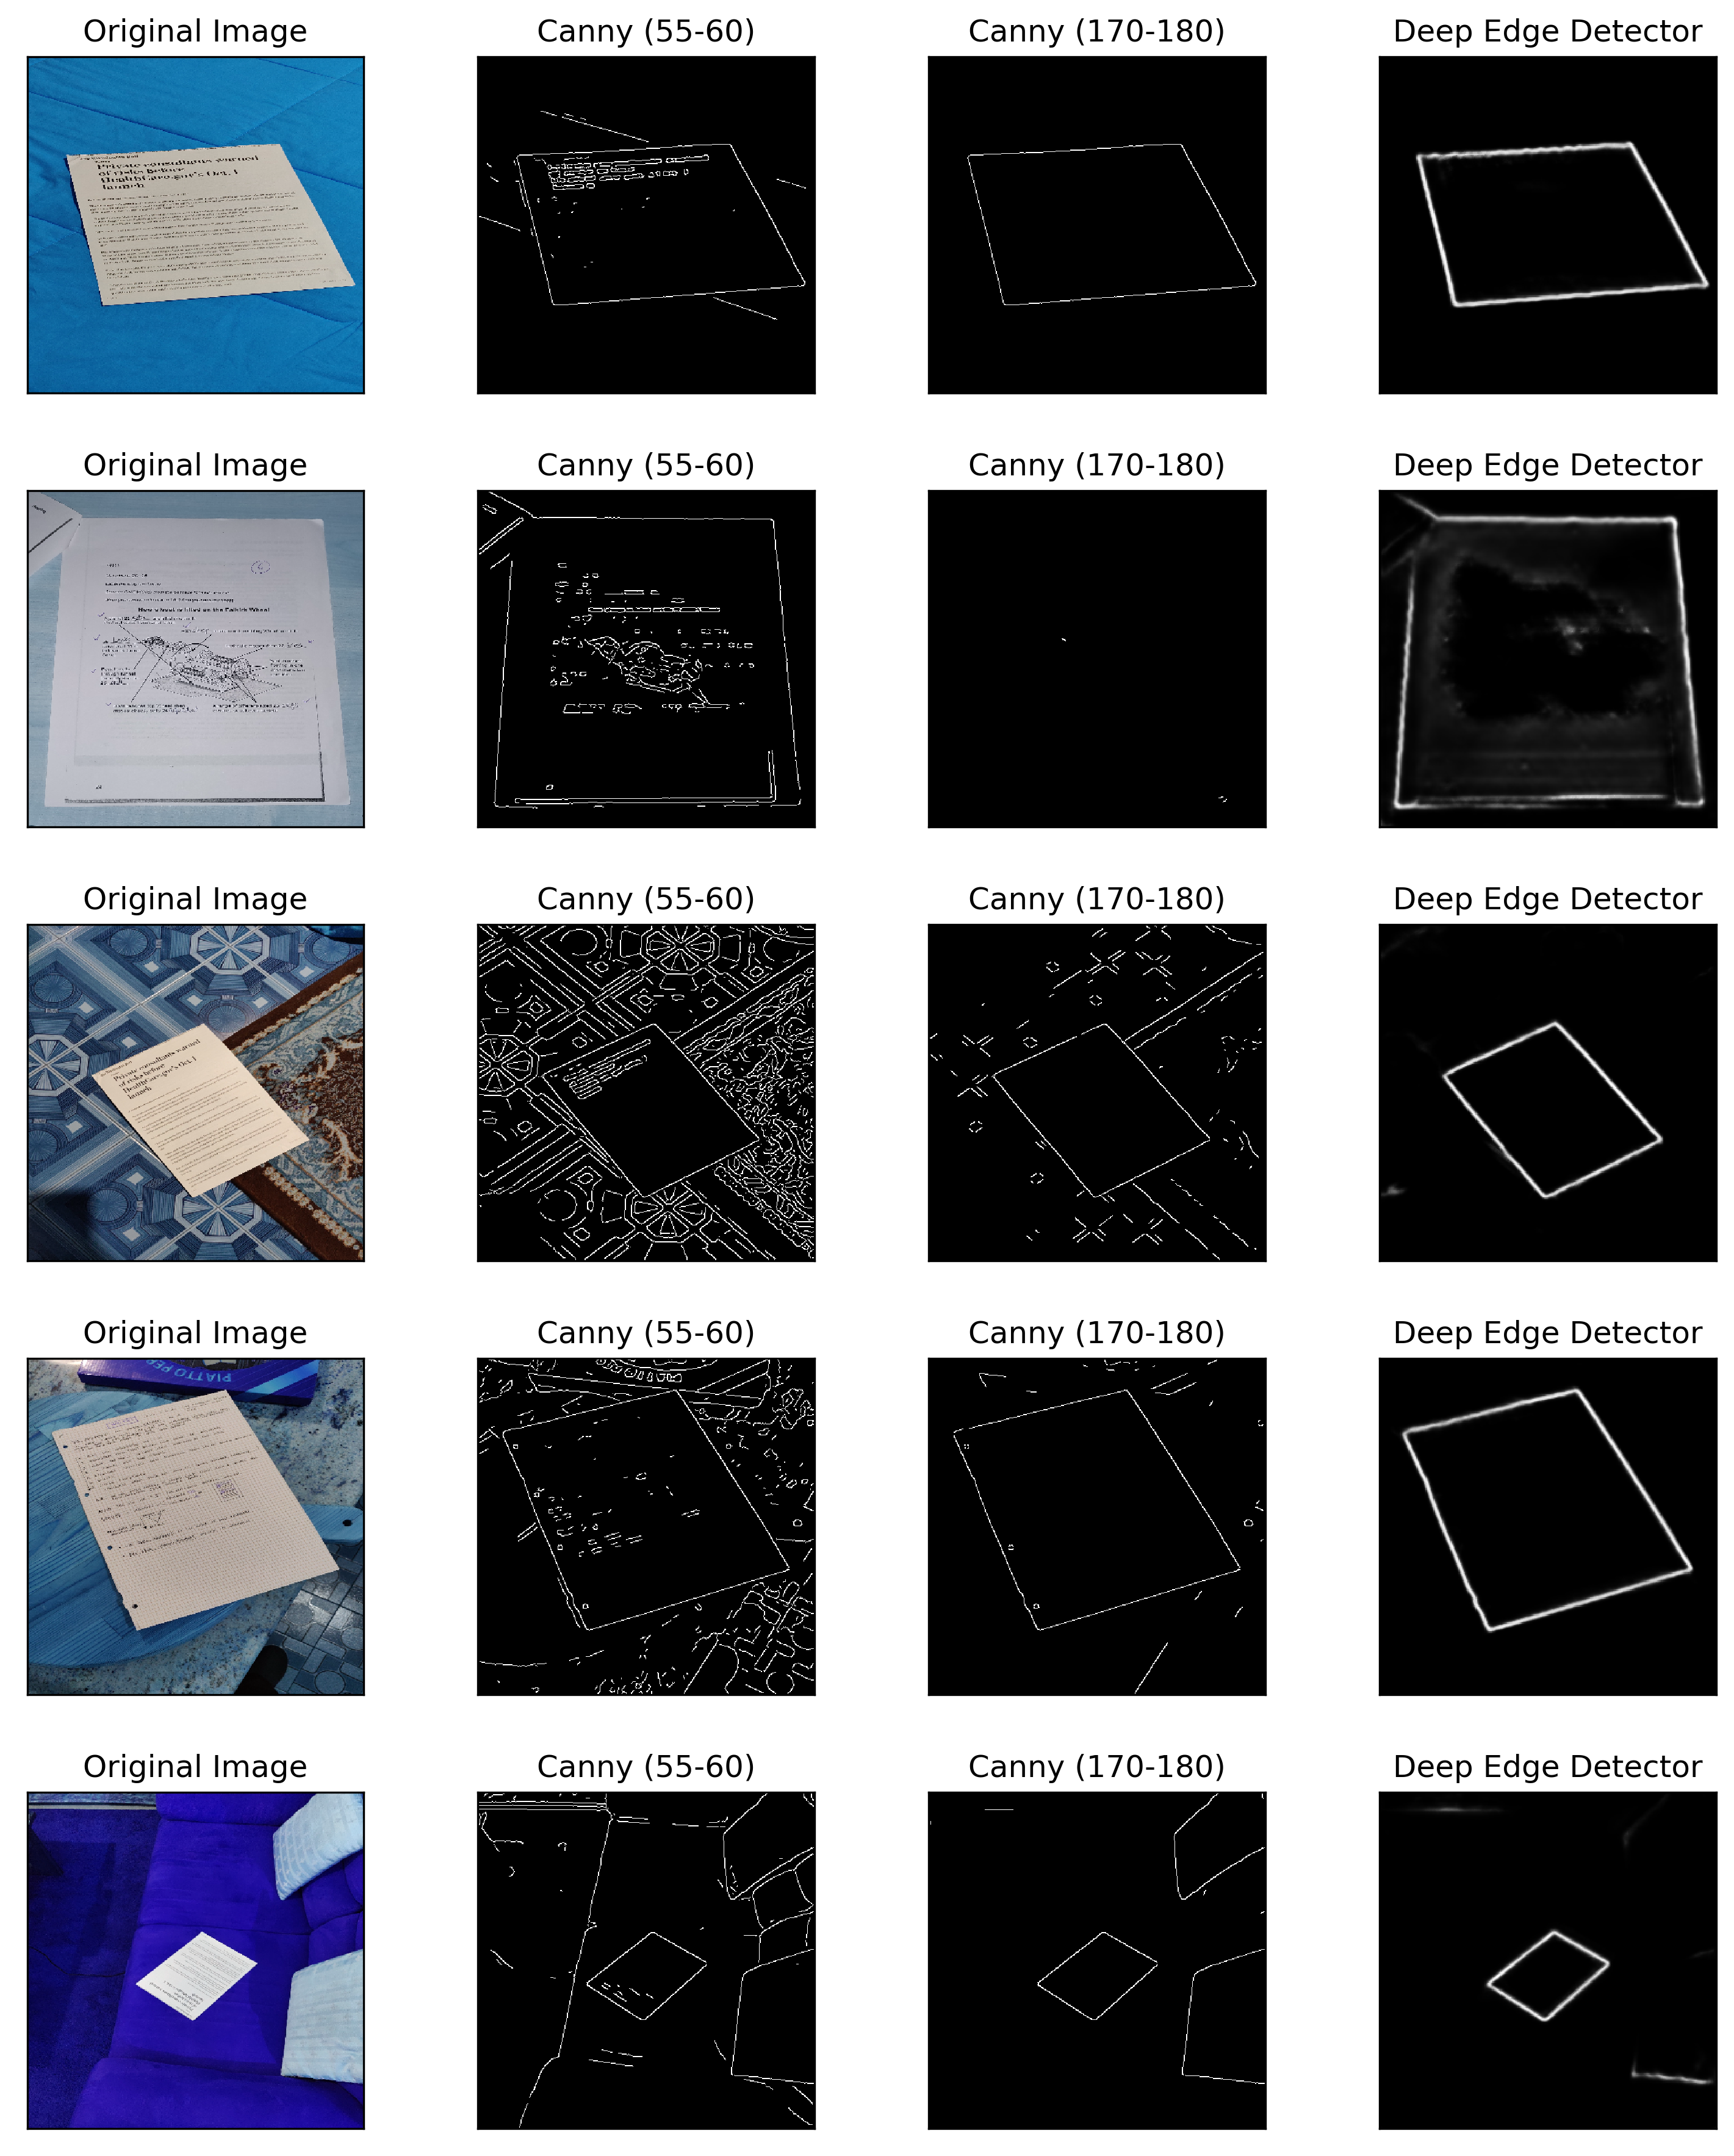
\includegraphics[width=1.2\textwidth]{deep_edge_comparison.png}}%

	\caption{Comparison of Canny and Deep Learning-based edge detection.}
	\label{fig:deep_comparison}
\end{figure}

\section{Corner detection}

The corner detection task goal is to find the four document corners starting from the one-channel edges image. These points should be as precise as possible in order to define the tightest convex polygon around the document. The intuitive method to solve this task is to use the Hough transformation, as suggested in a Dropbox article \footnote{https://blogs.dropbox.com/tech/2016/08/fast-and-accurate-document-detection-for-scanning/}, to find straight lines that best approximate the document edges; the corners will be the intersection between those lines.

The suggested method, relies on finding more than one line per edge resulting in a set of intersections points. Those points are used to compute polygons and the one which best approximate the document edges is chosen to define the four corners. However, from empirical experiments, this could lead to an high amount of intersections meaning an enormous amount of polygons to test. Instead, KODA implementation extracts the best four lines ahead, so their intersections are immediately the best corners.

All the operations described in the following section are computed with reference to the resized edges image which is by default 256x256.

\subsection{Hough Transform}

OpenCV provides an interface for computing Hough lines \footnote{https://docs.opencv.org/2.4/doc/tutorials/imgproc/imgtrans/hough\_lines/hough\_lines.html} using polar coordinates (rho, theta); the problem is to calibrate the parameters and select the best lines retrieved. In order to remove unwanted noise in the edges image, an intensity threshold, which value was determined empirically (80), is applied before submitting it to the OpenCV interface. The threshold and the resolution interface parameters also were found empirically. The input images come from a natural environment with no control of lighting, so it can be expected that edges images intensity may heavily varies. For this reason, if no Hough lines are found, the task iteratively tries to reduce the threshold parameter by 10\% until enough lines are found or a maximum number of iterations is reached (default is 3). 

Once a set of lines is found, a sub-task is responsible to select the four best ones, one per each document edge. This is accomplished exploiting the fact that the Hough lines returned by the OpenCV interface are ordered by confidence: the first four strongest ones are selected, as shown in Fig. \ref{fig:hough}.

\begin{figure}[H]
	\makebox[\textwidth][c]{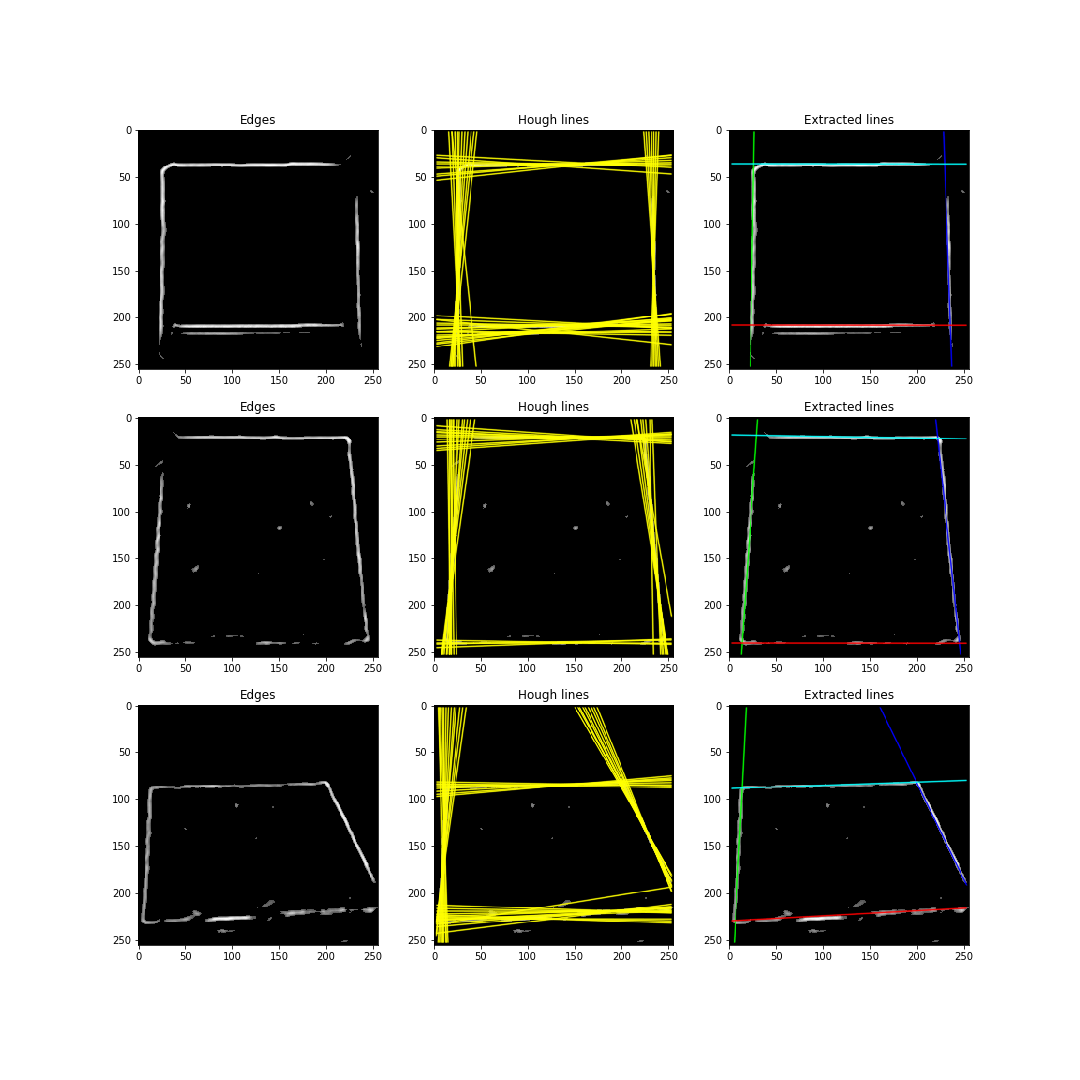
\includegraphics[width=1.2\textwidth]{Hough.png}}
	\caption{Hough lines computation extracting the best one per each document edge.}
	\label{fig:hough}
\end{figure}

\subsection{Computing corners}

Once the four Hough lines corresponding to the document edges are found, computing the document corners means to correctly intersect the lines. In order to distinguish lines that will be intersected from the others, they are sorted based on theta, so parallel lines are sequentially near to each other. In particular, the intersection is calculated as follow:

\begin{equation*}
	\begin{bmatrix} \cos(\sigma_1) & \sin(\sigma_1) \\ \cos(\sigma_2) & \sin(\sigma_2) \end{bmatrix}
	\begin{bmatrix} x \\ y \end{bmatrix}
	=
	\begin{bmatrix} \gamma_1 \\ \gamma_2 \end{bmatrix}
\end{equation*}
\begin{equation*}
	Ax = b
\end{equation*}

The implementation to find the intersection relies on \texttt{numpy.linalg.solve}\footnote{ \texttt{numpy.linalg.solve}: https://docs.scipy.org/doc/numpy/reference/generated/numpy.linalg.solve.html} which may raises an exception if the A matrix is singular because the computation is not possible. Whenever this happens, a least square solution, if it converges, via \texttt{numpy.linalg.lstsq} \footnote{\texttt{numpy.linalg.lstsq}: https://docs.scipy.org/doc/numpy/reference/generated/numpy.linalg.lstsq.html} is provided.

To maintain uniformity for the client API, the corners are sorted following the Cartesian quadrants and they are scaled up based on the original image size provided as input.

\begin{figure}[H]
	\makebox[\textwidth][c]{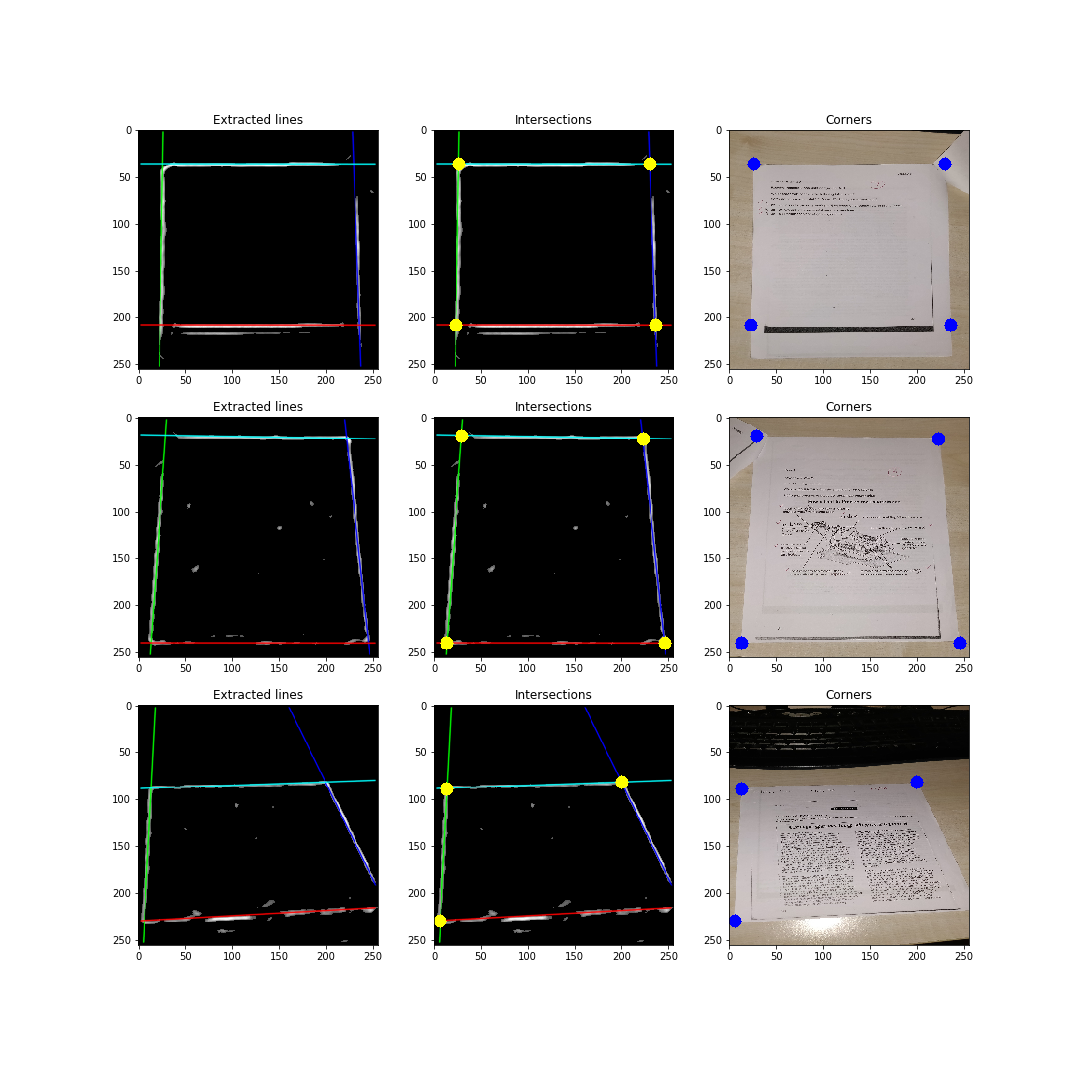
\includegraphics[width=1.2\textwidth]{computingcorners.png}}
	\caption{Computing corners as intersections of extracted Hough lines.}
	\label{fig:computingcorners}
\end{figure}

\section{Document analysis}

\subsection{Warping}

The first step of document analysis task is to warp the found paper within the image through a perspective transform using the detected corners. The document is expected to be A4 format, so the warped image size is computed considering the minimum of the possible widths (top, bottom) and heights (left, right), then forcing the greater dimension to be equals to the lesser one multiplied by the square root of 2 (ISO 216).

\begin{figure}[H]
	\makebox[\textwidth][c]{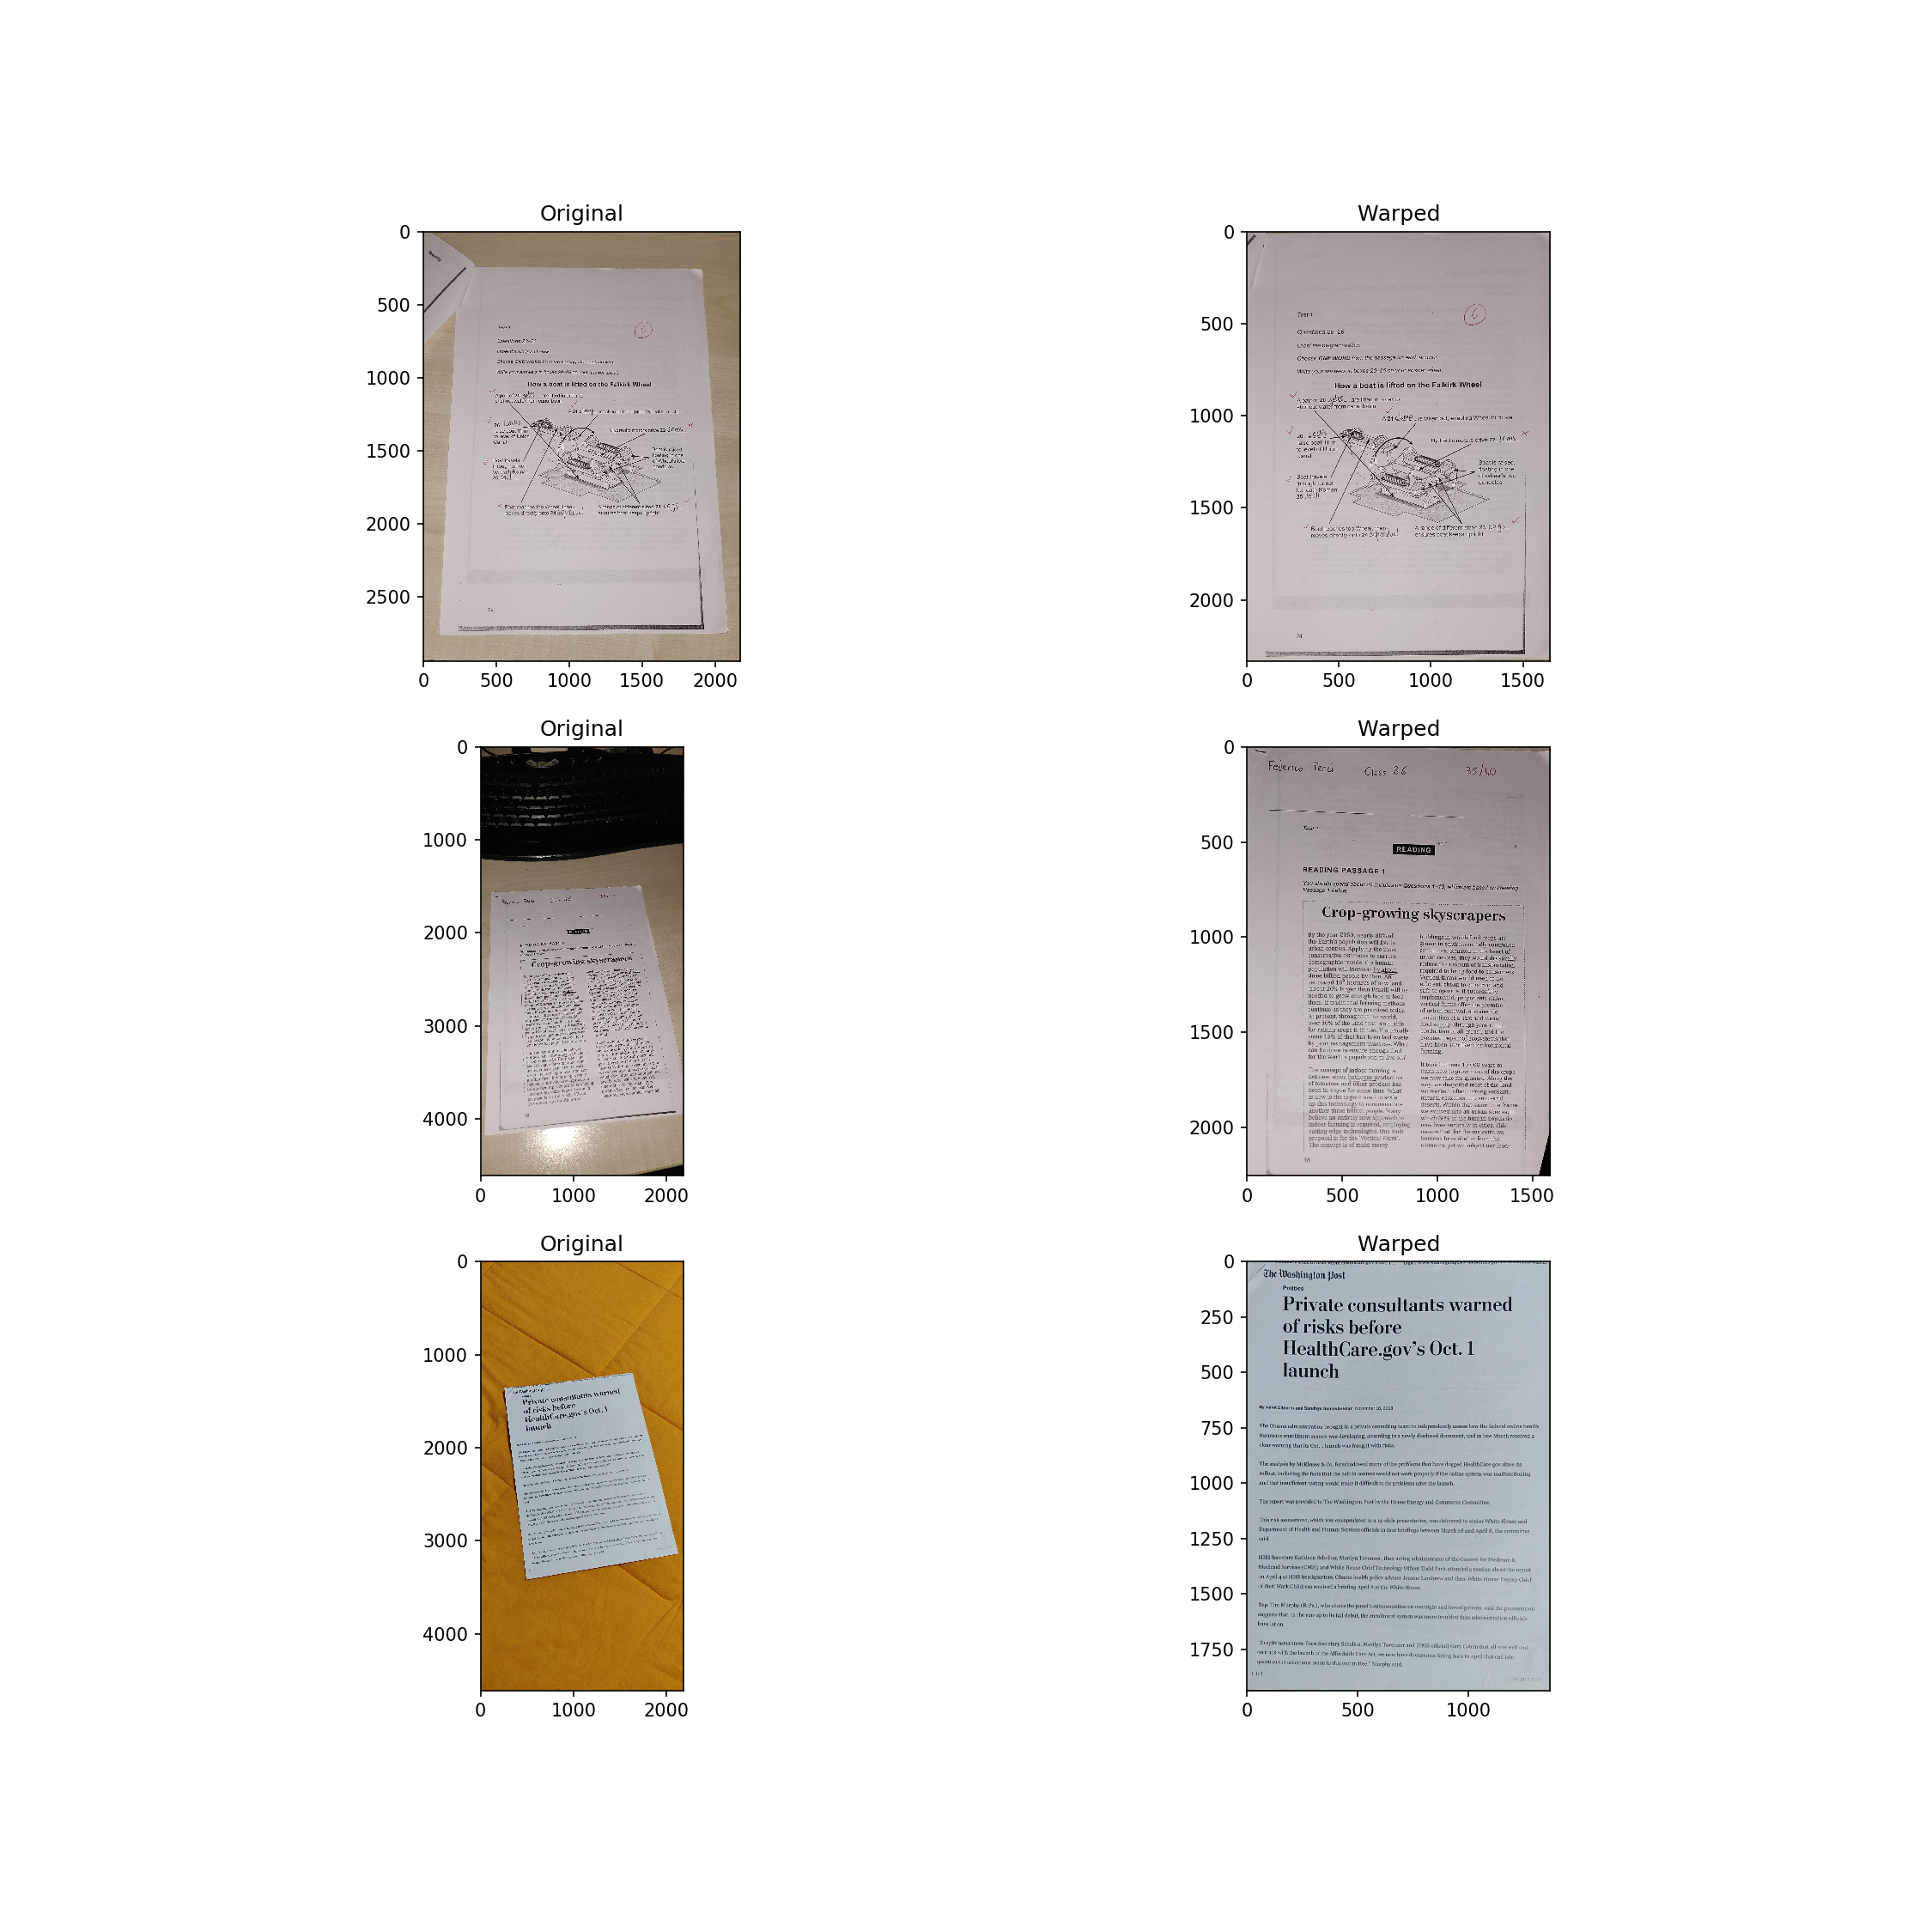
\includegraphics[width=1\textwidth]{Warping.png}}
	\caption{Comparison between original and warped images.}
	\label{fig:warping}
\end{figure}

\subsection{OCR}

In order to implement the \textit{Optical Character Recognition} feature needed to highlight keywords, KODA uses \textit{Tesseract}\footnote{https://github.com/tesseract-ocr/tesseract}, an open-source OCR engine by Google. Moreover, it uses \textit{TesserOCR}\footnote{https://github.com/sirfz/tesserocr}, a Python wrapper which provides a fast binding to the C++ native library and exposes all the low-level APIs.

Due to the keyword highlighting feature, it was crucial to get the position of single words rather than blocks of text. This is easily achieved using Tesseract's \textit{Iterators}, by setting the \textit{Page Iterator Level} to \texttt{WORD}. Thereafter, KODA can cycle through each word, filtering out the ones with low confidence and extracting the bounding boxes, as well as the text, as shown in Fig. \ref{fig:ocr}.

\begin{figure}[H]
	\makebox[\textwidth][c]{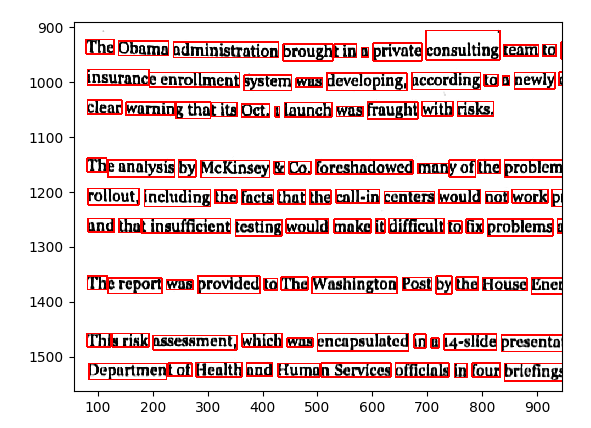
\includegraphics[width=1\textwidth]{ocr.png}}
	\caption{Example of OCR word segmenting}
	\label{fig:ocr}
\end{figure}

\subsection{Keyword highlighting}

The highlighting task goal is to apply a colored overlay on all the user specified keyword occurrences within the document in the image. Assuming the OCR library provides the bounding box of a detected word, a colored rectangle is drawn correspondingly on a image copy. The task output is the weighted sum of the original image and the overlay, resulting in a transparent highlighting effect on the keywords searched by the user. 

The formula applied \footnote{https://docs.opencv.org/2.4/modules/core/doc/operations\_on\_arrays.html} is formally as follow: %

\begin{equation}
	out = src_1 \cdot \alpha + src_2 \cdot \beta + \gamma
\end{equation}

Where:

\begin{center}
	$src_1$ = overlay image \\
	$src_2$ = original image \\
	$\alpha$ = 0.3  \\
	$\beta$ = 1 - $\alpha$ \\
	$\gamma$ = 0 
\end{center}

However, the OCR library performs on the warped image, instead of the original one. For this reason, the overlay has to be warped back to the document shape as in the original image. This requirement is satisfied by applying a perspective transformation using the inverse of the perspective transform matrix used to find the warped image. 

The KODA implementation (shown in Fig. \ref{fig:keywordhighliting}) relies on this concept, but actually transforms each bounding box instead of the entire final overlay. Transforming the warped image copy (final overlay) would lead to black pixels all over the areas where the document is not present: adding it to the orginal images results in darken areas outside the document. To avoid this problem, the highlights are drawn directly on the original image copy (not warped) after they are transformed correctly.

\begin{figure}[H]
	\makebox[\textwidth][c]{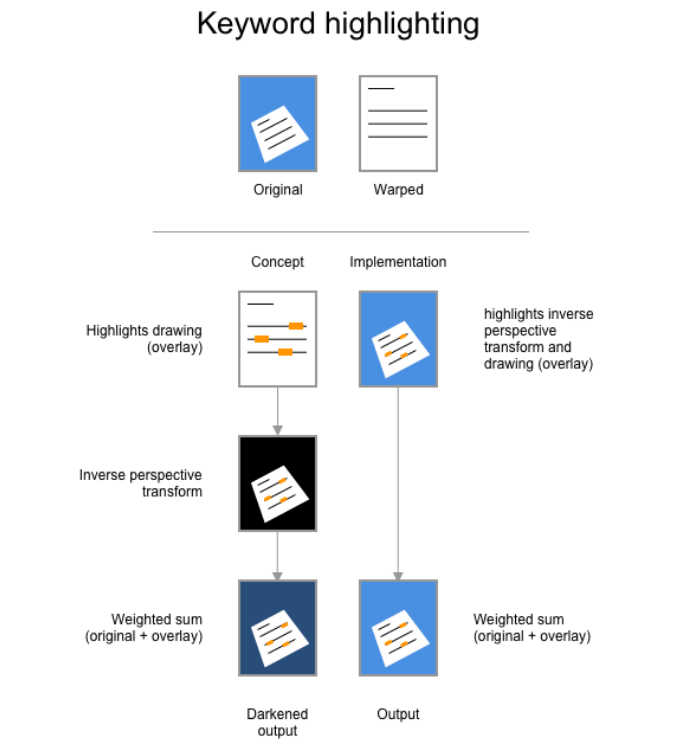
\includegraphics[width=1\textwidth]{kh.png}}
	\caption{Process to apply the highlight overlay.}
	\label{fig:keywordhighliting}
\end{figure}

\begin{figure}[H]
	\makebox[\textwidth][c]{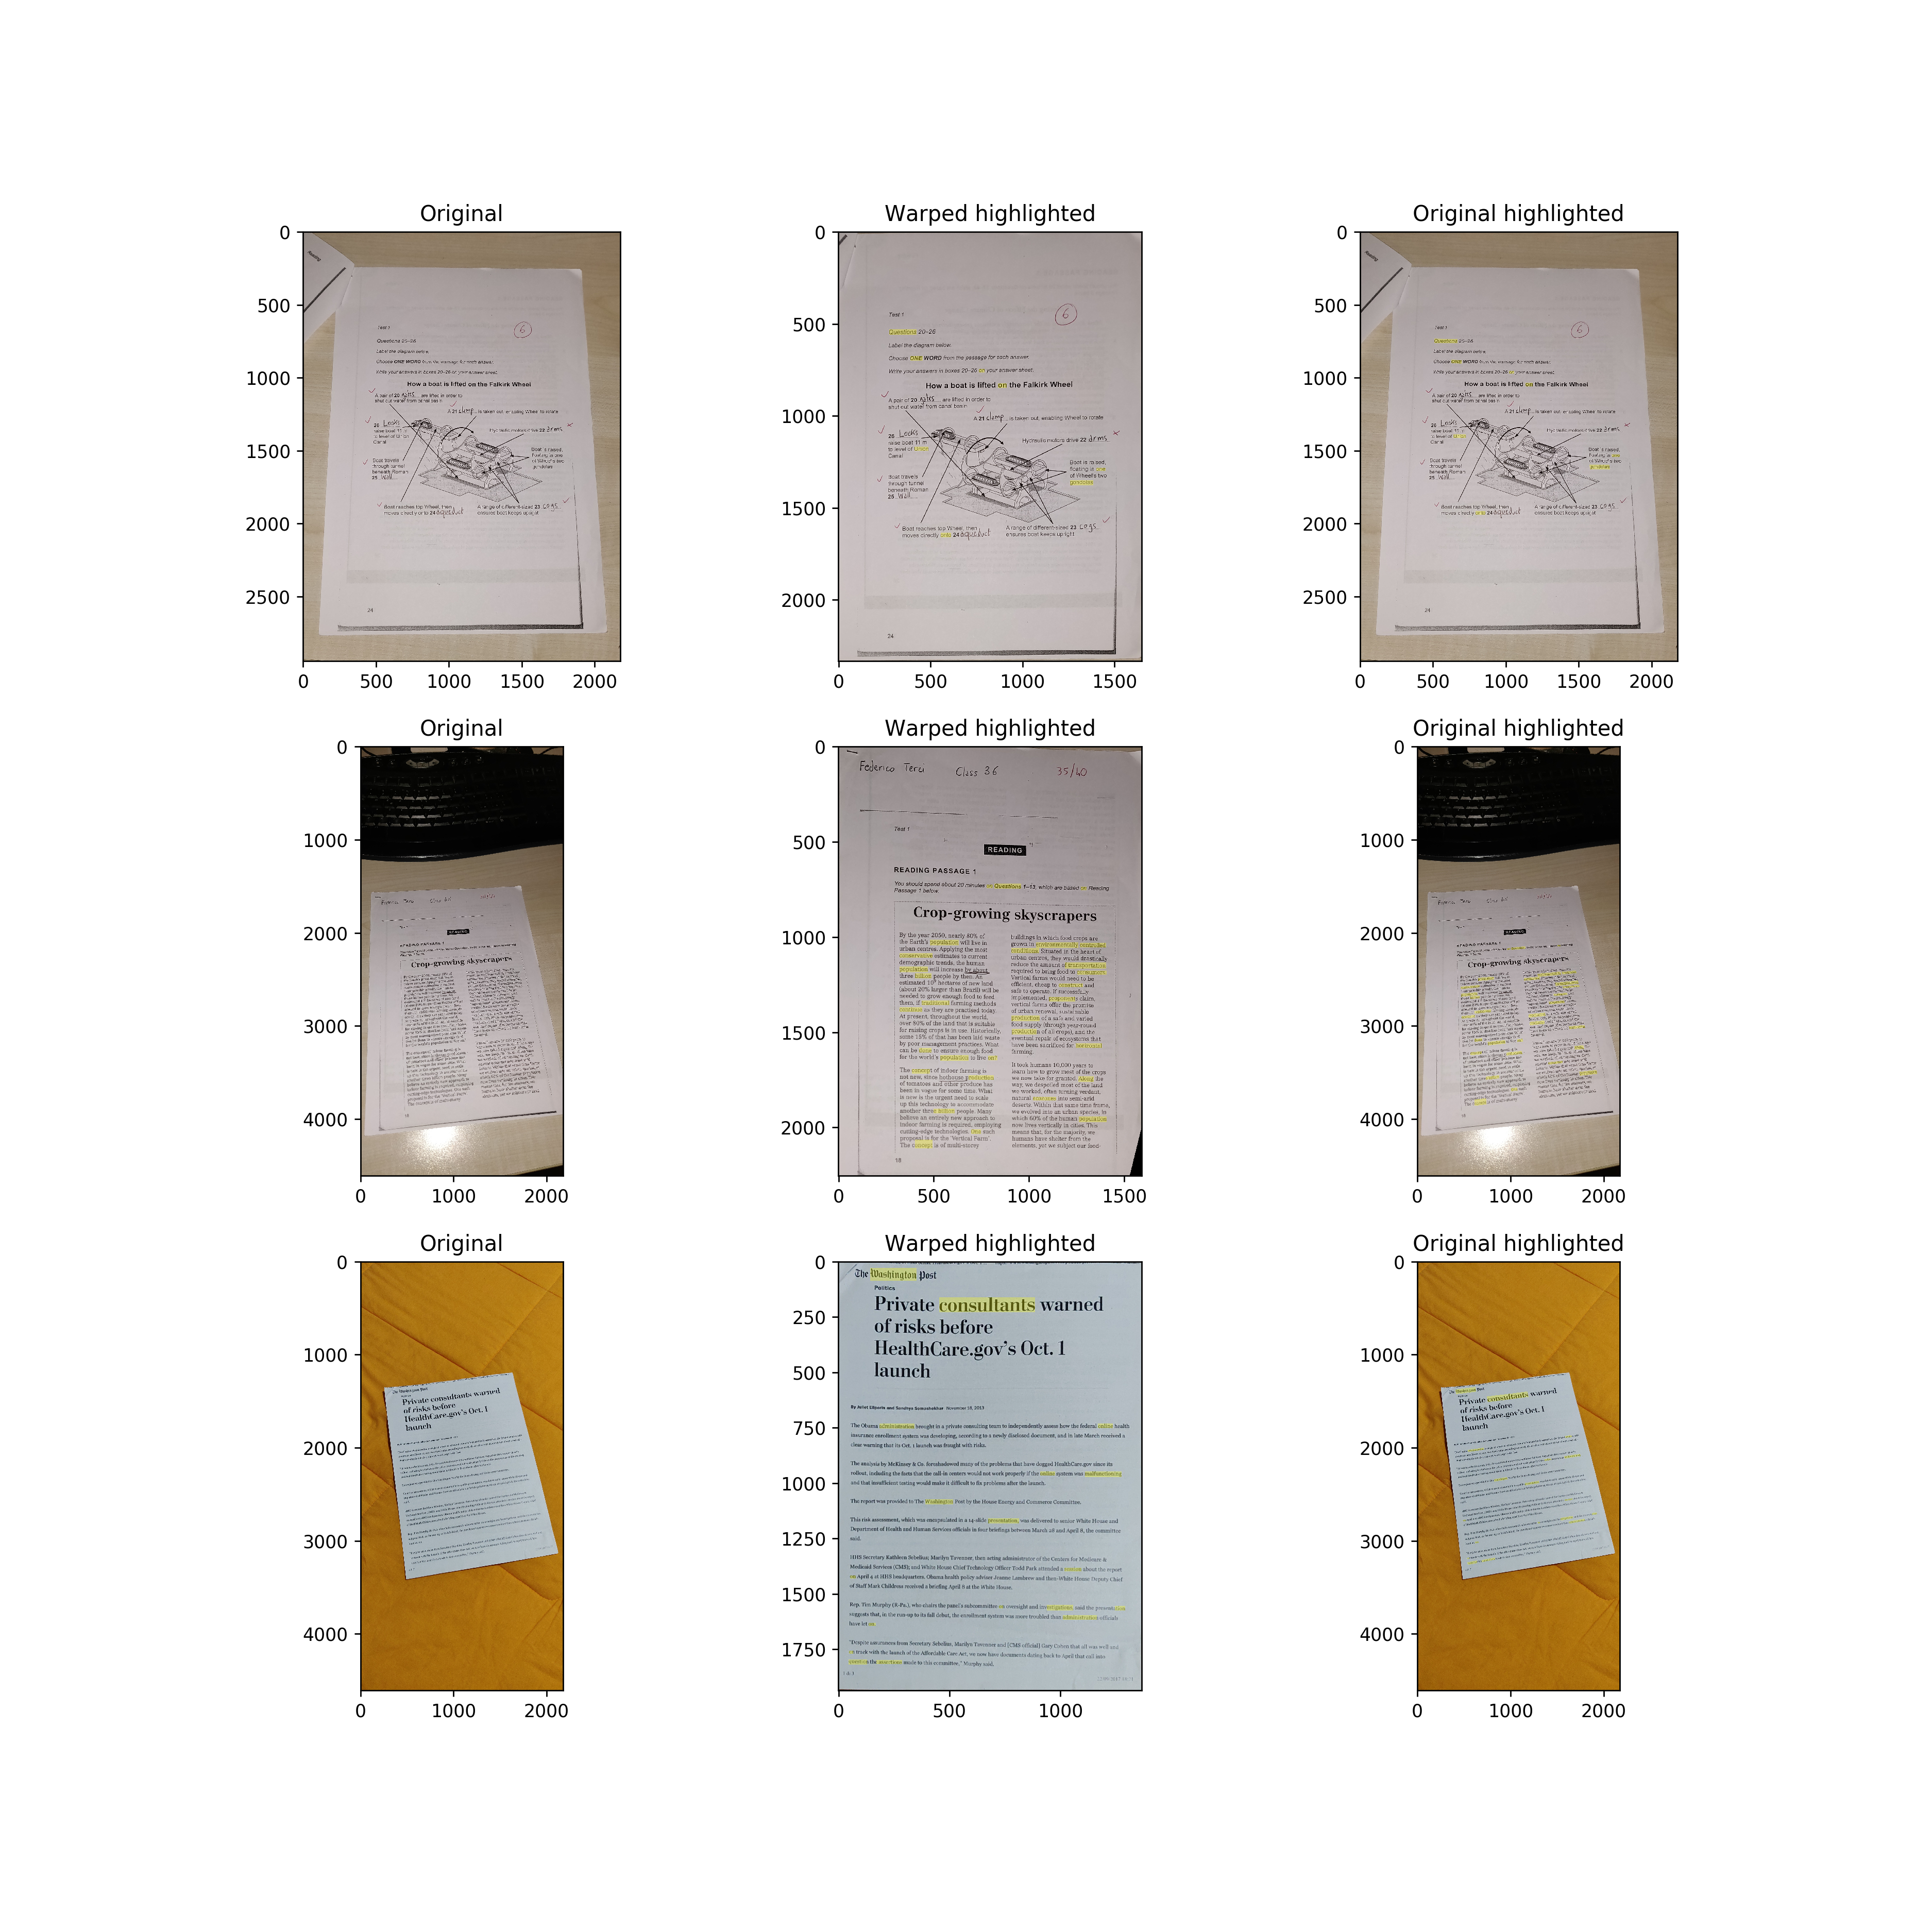
\includegraphics[width=1.5\textwidth]{Highlighting.png}}
	\caption{ Examples of the keyword "on" highlighting. Note: the keyword is not searched as a perfect match, but as a substring of actual words. The highlight is applied to the entire word.}
	\label{fig:keywordhighliting2}
\end{figure}

\section{Conclusion}

The proposed pipeline is able to correctly recognize and analyze the majority of document pictures in real-world scenarios, searching for the given keywords and preserving the original perspective, as shown in Fig. \ref{fig:result}.

\begin{figure}[H]
	\makebox[\textwidth][c]{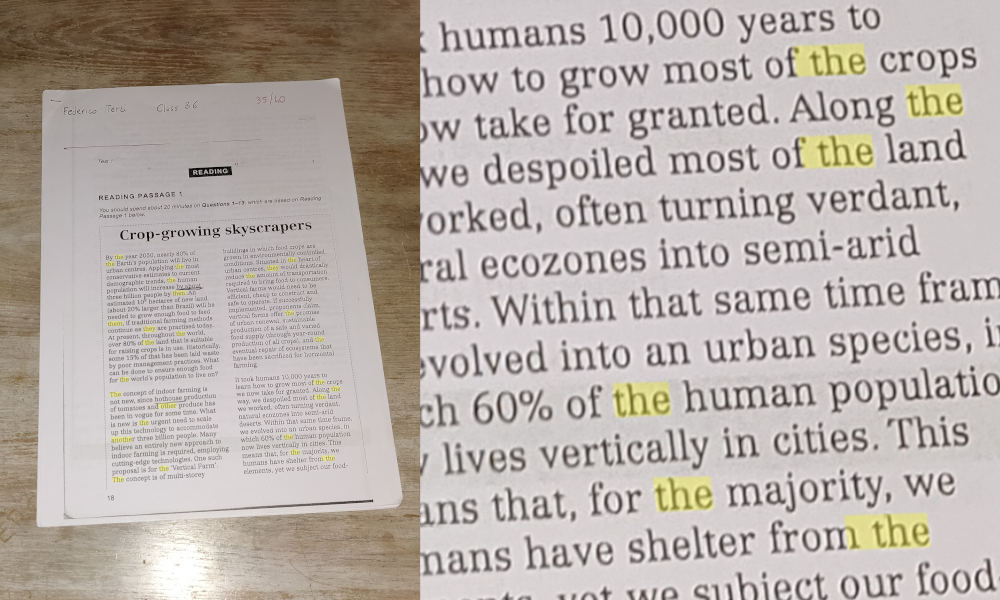
\includegraphics[width=1\textwidth]{result.png}}
	\caption{Example of KODA pipeline result for keyword "the". Overall output image on the left and close up on the right.}
	\label{fig:result}
\end{figure}

That said, KODA is still limited in certain situations. Firstly, the edge detection model was trained specifically to recognize white documents and, as a result, struggles with colored ones.
Moreover, although the deep learning-based edge detection offers superior results compared to traditional techniques, it is computationally expensive. In particular, the model itself weights about 360 megabytes and takes about 0.5/1 seconds to process the image on a modern desktop CPU, which makes it unsuitable for mobile applications.

Future improvements may focus on the creation of a less computationally and memory expensive edge detection, so that the pipeline can be ported on a mobile device.

\end{document}
